\documentclass{article}
\usepackage{arxiv}
\usepackage[utf8]{inputenc}
\usepackage[T1]{fontenc}
\usepackage{mathptmx}
\ifdefined\pdfgentounicode % pdfLaTeX (arXiv); tectonic/XeTeX skips this
  \input{glyphtounicode}\pdfgentounicode=1\pdfinterwordspaceon
\fi
\usepackage{microtype}
\emergencystretch=3em
\usepackage{amsmath, amssymb, amsthm, mathtools, bm}
\usepackage{graphicx, booktabs, array, float, placeins}
\graphicspath{{figures/}}
\usepackage{xcolor}
\usepackage[font=small, labelfont=bf, labelsep=period]{caption}
\usepackage{enumitem}
\setlist{itemsep=2pt, topsep=3pt}
\usepackage{tikz}
\usetikzlibrary{positioning, calc, arrows.meta}
\usepackage{listings}
\usepackage[round, authoryear]{natbib}
\usepackage[colorlinks=true, linkcolor=blue!45!black, citecolor=blue!45!black, urlcolor=blue!45!black]{hyperref}
\usepackage{xurl}
\hypersetup{pdftitle={Lockdowns as Partial Holidays}, pdfauthor={Thanatchon Chongmankhong},
  pdfkeywords={forecasting, calendar effects, Prophet, COVID-19, temporal aggregation, Thailand}}
\renewcommand{\shorttitle}{Lockdowns as Partial Holidays}

\theoremstyle{plain}
\newtheorem{proposition}{Proposition}
\newtheorem{corollary}{Corollary}
\theoremstyle{definition}
\newtheorem{assumption}{Assumption}
\renewcommand{\theassumption}{A\arabic{assumption}}
\newtheorem{definition}{Definition}
\theoremstyle{remark}
\newtheorem{remark}{Remark}
\newcommand{\HESI}{\mathrm{HESI}}
\newcommand{\E}{\mathbb{E}}
\lstset{language=Python, basicstyle=\ttfamily\scriptsize, keywordstyle=\color{blue!60!black}\bfseries,
  commentstyle=\color{green!40!black}\itshape, stringstyle=\color{red!50!black}, frame=single,
  rulecolor=\color{black!25}, breaklines=true, columns=fullflexible, showstringspaces=false,
  backgroundcolor=\color{black!2}}

\title{Lockdowns as Partial Holidays:\\ Identifying Work-Stoppage Elasticities from Recurring Holidays and Transferring Them to Forecast Thailand's Monthly Exports through the COVID-19 Shock}
\author{\textbf{Thanatchon Chongmankhong}}
\date{November 7, 2026}

\begin{document}
\maketitle



\begin{abstract}
\noindent The COVID-19 pandemic produced a collapse-and-rebound episode in Thailand's monthly export series that contaminates the trend and seasonal components learned by forecasting models and, more fundamentally, cannot be anticipated by any parameter estimated before the shock. This paper proposes the \emph{Holiday-Equivalent Stoppage} (HES) framework, which treats a lockdown as a partial holiday. Recurring holidays---Thai public holidays including Songkran (domestic channel) and the Chinese New Year window (partner channel)---identify a work-stoppage elasticity through one \emph{shared} regressor per channel in a decomposable forecasting model (Prophet). The elasticity is transferred to the pandemic through a Holiday-Equivalent Stoppage Index (HESI) that expresses each lockdown day in holiday units, computed as the drop in workplace mobility relative to its drop on actual holidays. We derive (i) an error decomposition showing that the transfer is exact when the dose is correctly scaled and that calibration absorbs the projection of unmodelled shocks on the dose path; (ii) a Jensen-type aggregation bias under which monthly models attenuate a daily elasticity $\beta$ to approximately $e^{\beta}-1$; (iii) the resulting identification problem with monthly data together with a closed-form aggregation correction; and (iv) dose saturation in tree ensembles. A Monte Carlo study with <<nseeds>> replications, in which export values are simulated while the holiday calendar and the OxCGRT and Google Mobility data are real, confirms each prediction. With a correctly scaled dose, daily Prophet reduces the 2020--2021 mean absolute percentage error (MAPE) from <<e1.s1.pd.off.w24>>\% to <<e1.s1.pd.hesi.w24>>\%, whereas switching holiday effects on for whole months (<<e1.s1.pd.binary.w24>>\%) or using raw stringency (<<e1.s1.pd.stringency.w24>>\%) does not help. Daily estimation recovers the elasticity ($<<bD.pd>>$ against a true $<<bD.true>>$), monthly estimation yields $<<bD.pm>>$, close to the predicted $e^{\beta}-1=<<bM.closed>>$, and LightGBM saturates. After the shock, SARIMAX and simply masking the shock window remain competitive. HES is therefore a structured tool for measurable stoppage shocks rather than a universal accuracy improvement.
\end{abstract}

\keywords{Forecasting under structural shocks \and Calendar effects \and Prophet \and COVID-19 \and Temporal aggregation \and Tree ensembles \and International trade \and Thailand}

\noindent{\bfseries\emph{JEL codes}}\enspace C15, C22, C53, F17

\section{Introduction}\label{sec:intro}
Thailand is among the most trade-dependent economies in Asia, and its monthly merchandise-export statistics are one of the most closely watched indicators of the business cycle. They are forecast routinely by government agencies, the central bank and private institutions, typically with univariate or calendar-augmented time-series models and, increasingly, with machine-learning methods. The COVID-19 pandemic confronted all of these models with an episode unlike anything in their estimation samples: a sharp contraction in the second quarter of 2020, followed by a rebound in 2021 that was driven at least as much by global demand as by the lifting of domestic restrictions \citep{baldwin2020trade}. Episodes of this kind are a principal source of forecast failure \citep{clements1998forecasting, rossi2013instability}.

Such episodes create three distinct problems. The first is \emph{contamination}: models that learn trend and seasonal components from the data absorb the shock into these components, so forecasts made after the shock inherit its distortions. The second is \emph{propagation}: lagged features carry the anomaly forward, so a collapse in 2020 depresses forecasts for 2021 through year-on-year lags. The third, and most fundamental, is \emph{unforecastability}: a model has no parameter describing the effect of a lockdown until a lockdown has been observed. The first two problems concern estimation after a shock; the third concerns forecasting during one.

The literature offers many tools for the first two problems: intervention analysis \citep{box1975intervention}, joint estimation of outlier effects \citep{chen1993joint}, structural-break estimation \citep{bai1998multiple}, estimation-window selection \citep{pesaran2007window}, volatility rescaling of vector autoregressions after March 2020 \citep{lenza2022var}, and analogue forecasting based on earlier recessions \citep{foroni2022covid}. Practitioners using Prophet are advised to encode lockdown periods as one-off holidays \citep{prophetshocks}. All of these remedies identify the effect of a shock \emph{after} observing it. Tree ensembles, which dominate recent forecasting competitions \citep{makridakis2022m5}, face an additional obstacle: their prediction functions are piecewise constant and cannot extrapolate beyond the support of the training data \citep{hastie2009elements, januschowski2022trees}.

This paper starts from a simple observation. From the point of view of production and shipping, a lockdown resembles a holiday: factories, offices, ports and customs operate at reduced capacity because people do not go to work. Thailand runs a natural experiment of this kind every year. Songkran, the Thai New Year in mid-April, and the other public holidays close large parts of the economy for one to five days, and the Chinese New Year closes Thailand's largest trading partner for about a week. These events recur in every year of a pre-pandemic sample, so their effect on exports is identified long before the pandemic. If the intensity of a lockdown could be expressed in holiday units---``a lockdown day is equivalent to 0.3 of a holiday''---the holiday elasticity would deliver a forecast of the lockdown effect without any new parameter.

The naive implementation of this idea, switching the holiday effect on for every day of a lockdown month, implicitly assumes that a lockdown day is a full holiday, which is rarely true. We therefore replace the switch with a \emph{dose}: the Holiday-Equivalent Stoppage Index (HESI), defined as the drop in workplace mobility on a given day divided by the typical drop on a public holiday, both measured in the Google Community Mobility Reports \citep{google2022mobility}. The holiday serves as the unit of measurement that converts mobility into stoppage. We address five research questions:
\begin{enumerate}[label=\textbf{RQ\arabic*}, leftmargin=3.2em]
\item \emph{Transfer.} Can an elasticity identified from recurring holidays forecast exports during lockdowns that never occur in the estimation sample?
\item \emph{Dose.} How sensitive is the transfer to the scale of the dose, and can the scale be calibrated in real time?
\item \emph{Frequency.} What is lost when only monthly data are available, and can it be recovered?
\item \emph{Model class.} Can tree ensembles perform the same transfer?
\item \emph{Aftermath.} How should the shock be treated when forecasting after it has ended?
\end{enumerate}

The paper makes four contributions. First, it formulates the HES framework, in which one shared regressor per channel carries both recurring holidays and pandemic doses, and it makes the identifying assumptions explicit. Second, it derives the theoretical properties of the framework: an error decomposition with an explicit optimal dose; a Jensen-type aggregation bias with the closed form $e^{\beta}-1$; a closed-form aggregation correction with its delta-method variance; the identification problem of monthly data; the dose saturation of tree ensembles; and the reason why one-off holidays cannot transfer. Third, it evaluates the framework in a Monte Carlo study designed according to the ADEMP structure of \citet{morris2019simulation}, built on the real Thai holiday calendar and on real policy and mobility data, with paired inference across replications. The theory predicts the simulation outcomes quantitatively, not only qualitatively. Fourth, it provides an open implementation and a protocol for official export statistics.

The main findings are as follows. With a correctly scaled dose, transfer works: daily Prophet reduces the 2020--2021 MAPE from <<e1.s1.pd.off.w24>>\% to <<e1.s1.pd.hesi.w24>>\% without observing a single pandemic day, and it improves on the no-dose forecast in <<win.s1.hesi.off>>\% of replications. The whole-month switch and raw stringency do not help. When the mobility dose overstates the true stoppage two-fold, calibrating the scale on the first two lockdown months lowers the average MAPE from <<e1.s2.pd.off.w20>>\% to <<e1.s2.pd.cal.w20>>\% and significantly improves on the uncalibrated dose, although the gain over the no-dose forecast is not consistent enough across replications to survive a multiple-testing correction. Monthly estimation attenuates the elasticity almost exactly as predicted, and the aggregation correction removes the bias at the cost of a variance that the delta method also predicts. Tree ensembles switch rather than dose. After the shock, a simple SARIMAX model and masking the shock window are at least as accurate as HES, and in normal times tree ensembles are the most accurate method.

All quantitative results in this paper come from a simulation study; applying the framework to official Thai export statistics, which the accompanying code supports, is left for future work.

Section~\ref{sec:lit} reviews related work. Section~\ref{sec:framework} presents the framework and Section~\ref{sec:theory} its theoretical properties. Section~\ref{sec:design} describes the simulation design and Section~\ref{sec:results} the results. Section~\ref{sec:discussion} discusses implications, threats to validity and a protocol for official data, and Section~\ref{sec:conclusion} concludes. Proofs are collected in Appendix~\ref{app:proofs}.

\section{Related literature}\label{sec:lit}
\paragraph{Calendar and moving-holiday effects.} The modelling of trading-day and holiday effects in monthly series has a long tradition in official statistics. \citet{cleveland1982calendar} and \citet{bell1983calendar} formulate regression models for calendar variation, and moving-holiday regressors for festivals such as Easter became a standard component of X-12-ARIMA \citep{findley1998x12}. For Asian economies, the Lunar New Year shifts between January and February and induces large month-to-month swings that require dedicated regressors \citep{lin2003lunar}. This literature estimates holiday effects in order to remove them; we estimate them in order to \emph{reuse} them as a source of identifying variation for a different shock.

\paragraph{Structural change, interventions and forecast failure.} Intervention analysis \citep{box1975intervention} and the joint estimation of outlier effects \citep{chen1993joint} model known or detected disturbances with dummy-type regressors whose coefficients are estimated from the disturbance itself. Tests and estimators for structural breaks \citep{perron1989crash, bai1998multiple}, evidence of pervasive instability \citep{stock1996instability} and the theory of forecast failure \citep{clements1998forecasting, rossi2013instability} explain why such disturbances degrade forecasts, and estimation-window selection \citep{pesaran2007window} offers one response. In all of these approaches the size of the disturbance is learned from the disturbance; none provides a forecast of its effect before it is observed.

\paragraph{Forecasting through the pandemic.} \citet{lenza2022var} show how to estimate vector autoregressions after March 2020 by rescaling shock volatility, and \citet{foroni2022covid} use the dynamics of the Global Financial Crisis to forecast the COVID-19 recession and recovery. Both rely on similarity of \emph{magnitude} with earlier events. Our approach relies on similarity of \emph{mechanism} with events that recur every year. On the trade side, \citet{baldwin2020trade} emphasise that the pandemic hit trade through supply disruptions, demand collapse and supply-chain contagion; HES targets the first channel and treats the others as unmodelled shocks, a distinction that matters for calibration (Proposition~\ref{prop:transfer}).

\paragraph{Decomposable models and Prophet.} Prophet \citep{taylor2018forecasting} represents a series as the sum of a piecewise-linear trend, Fourier seasonality, holiday effects and extra regressors, estimated by maximum a posteriori under Gaussian and Laplace priors; see also \citet{hyndman2021fpp} for a textbook treatment of related decompositions. Each holiday name receives its own coefficients, which is convenient for seasonal holidays but implies that a new ``COVID'' holiday has no information before it occurs (Remark~\ref{rem:oneoff}).

\paragraph{Tree ensembles.} Regression trees \citep{breiman1984cart} and gradient boosting \citep{friedman2001greedy}, in particular LightGBM \citep{ke2017lightgbm}, are among the most accurate methods for tabular data \citep{grinsztajn2022tree} and in large forecasting competitions \citep{makridakis2022m5}. Their prediction functions are piecewise constant and flat outside the training support \citep{hastie2009elements, januschowski2022trees}. We show that this property prevents them from transferring a dose even when the dose variable is supplied explicitly.

\paragraph{Temporal aggregation and mixed frequency.} The effects of temporal aggregation on time-series models are surveyed by \citet{silvestrini2008aggregation}; temporal disaggregation \citep{chow1971interpolation, denton1971adjustment} and mixed-data-sampling regressions \citep{ghysels2007midas} address the mismatch between high- and low-frequency information. We add a specific result: under a log link, holiday effects concentrated on a few days and lockdown effects spread over a month aggregate differently, which biases monthly estimates of a daily elasticity in a predictable way.

\paragraph{Policy and mobility data.} The Oxford COVID-19 Government Response Tracker \citep{hale2021oxcgrt} provides daily stringency indices, and the Google Community Mobility Reports \citep{google2022mobility} provide daily changes in visits to workplaces and other places relative to a pre-pandemic baseline. Mobility data have been used to nowcast economic activity \citep{sampi2020nowcasting}. We use them in a different role: as a unit converter between lockdown intensity and holiday-equivalent stoppage.

\section{The Holiday-Equivalent Stoppage framework}\label{sec:framework}
\subsection{Setup and notation}
Let $d$ index calendar days and $m$ months, let $y_d$ denote the value of exports on day $d$, $Y_m=\sum_{d\in m}y_d$ the monthly total and $D_m$ the number of days in month $m$. Let $H_d=1$ if $d$ is an \emph{observed} Thai public holiday, including in-lieu and special holidays (for example, the 2020 Songkran holiday was postponed and replaced by 27 July, 4 September and 7 September 2020), and $C_d=1$ if $d$ lies in the Chinese-New-Year window $[\tau_y-1,\tau_y+6]$, where $\tau_y$ is the first day of the Spring Festival in year $y$. The daily model is
\begin{equation}\label{eq:model}
\log y_d \;=\; g(t_d) + s(t_d) + w(d) + \beta_D\,x^D_d + \beta_P\,x^P_d + D_d + u_d ,
\end{equation}
where $g$ is a piecewise-linear trend, $s$ a Fourier representation of yearly seasonality, $w$ a day-of-week effect, $D_d$ an unobserved non-stoppage shock (for instance, a collapse of foreign demand) and $u_d$ a stationary disturbance.

\subsection{Shared stoppage regressors}
\begin{definition}[Shared stoppage regressors]\label{def:shared}
Given a domestic dose $h_d\in[0,1]$, a partner dose $p_d\in[0,1]$ and a dose multiplier $\lambda>0$,
\begin{align}
x^D_d &= H_d + (1-H_d)\,\min\{1,\ \lambda h_d\}, \label{eq:xd}\\
x^P_d &= C_d + (1-C_d)\,p_d . \label{eq:xp}
\end{align}
\end{definition}
The defining feature is that $\beta_D$ and $\beta_P$ multiply \emph{both} the recurring holiday indicators and the pandemic doses. Before 2020 the doses are zero, so $x^D_d=H_d$ and $x^P_d=C_d$, and the elasticities are identified from about a decade of holidays. During the pandemic, the forecast requires only the doses; no new parameter is introduced. Figure~\ref{fig:framework} summarises the structure.

\begin{figure}[t]
\centering
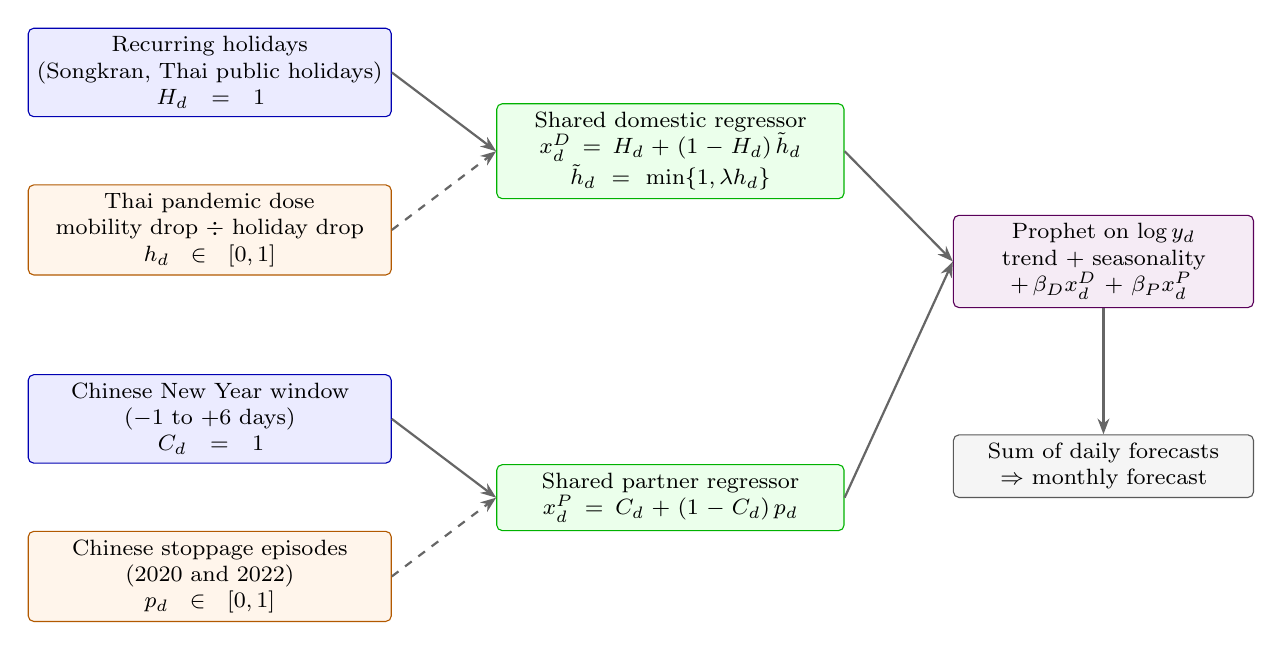
\begin{tikzpicture}[x=1mm, y=1mm, every node/.style={font=\footnotesize},
  box/.style={draw=#1!70!black, fill=#1!8, rounded corners=2pt, align=center, inner sep=3pt},
  arr/.style={-{Stealth[length=2mm]}, thick, draw=black!60}]
\node[box=blue,   text width=44mm] (hol) at (23.5,   0)  {Recurring holidays\\(Songkran, Thai public holidays)\\$H_d=1$};
\node[box=orange, text width=44mm] (cov) at (23.5, -20)  {Thai pandemic dose\\mobility drop $\div$ holiday drop\\$h_d\in[0,1]$};
\node[box=blue,   text width=44mm] (cny) at (23.5, -44)  {Chinese New Year window\\($-1$ to $+6$ days)\\$C_d=1$};
\node[box=orange, text width=44mm] (cn)  at (23.5, -64)  {Chinese stoppage episodes\\(2020 and 2022)\\$p_d\in[0,1]$};
\node[box=green,  text width=42mm] (xd)  at (82, -10)  {Shared domestic regressor\\$x^D_d=H_d+(1-H_d)\,\tilde h_d$\\$\tilde h_d=\min\{1,\lambda h_d\}$};
\node[box=green,  text width=42mm] (xp)  at (82, -54)  {Shared partner regressor\\$x^P_d=C_d+(1-C_d)\,p_d$};
\node[box=violet, text width=36mm] (pr)  at (137, -24) {Prophet on $\log y_d$\\trend + seasonality\\$+\,\beta_D x^D_d+\beta_P x^P_d$};
\node[box=gray,   text width=36mm] (out) at (137, -50) {Sum of daily forecasts\\$\Rightarrow$ monthly forecast};
\draw[arr] (hol.east) -- (xd.west);
\draw[arr, dashed] (cov.east) -- (xd.west);
\draw[arr] (cny.east) -- (xp.west);
\draw[arr, dashed] (cn.east) -- (xp.west);
\draw[arr] (xd.east) -- (pr.west);
\draw[arr] (xp.east) -- (pr.west);
\draw[arr] (pr.south) -- (out.north);
\end{tikzpicture}
\caption{The HES framework. \emph{Colour key:} blue boxes are the recurring holidays that identify the elasticities before the pandemic; orange boxes are the dose inputs measured during the pandemic; green boxes are the shared regressors that carry both; the violet box is the forecasting model and the grey box the monthly output. Solid arrows: the holiday indicators that identify $\beta_D$ and $\beta_P$; dashed arrows: dose inputs that enter the same regressors during the pandemic.}
\label{fig:framework}
\end{figure}

\subsection{Measuring the dose: the Holiday-Equivalent Stoppage Index}
Let $m_d=\max\{0,-\text{workplaces}_d/100\}$ be the proportional drop in visits to workplaces relative to the pre-pandemic baseline in the Google Community Mobility Reports, and let $\mathcal{H}^{wd}$ be the set of public holidays that fall on weekdays. The domestic dose is
\begin{equation}\label{eq:hesi}
h_d \;=\; \min\Bigl\{1,\ \frac{\tilde m_d}{\operatorname{med}\{m_e: e\in\mathcal{H}^{wd}\}}\Bigr\},
\end{equation}
where $\tilde m_d$ is a seven-day centred moving average computed after removing holidays, so that holiday dips do not leak into neighbouring days. In the Thai data from 15 February 2020 to 19 August 2022 there are 57 weekday holidays with a median drop of <<mobref>> (Figure~\ref{fig:drivers}a); Songkran and New Year days are stronger, at 0.64--0.70. The average of $h_d$ in April 2020 is 0.60: in terms of attendance at workplaces, a day of the April 2020 lockdown was equivalent to six tenths of a holiday.

Workplace attendance is not export production. Office work can move home while export-oriented factories, typically designated as essential, keep operating. We therefore model the \emph{true} stoppage dose as
\begin{equation}\label{eq:measurement}
z_d = \kappa\, h_d\,(1+\nu_d),
\end{equation}
where $\kappa>0$ is an unknown pass-through and $\nu_d$ a mean-zero, slowly varying proxy error. The multiplier $\lambda$ in~\eqref{eq:xd} is the forecaster's choice for $\kappa$.

For the partner channel, policy stringency is not a measure of stoppage. Under China's zero-COVID policy the OxCGRT index stayed between 0.6 and 0.8 for three years while most factories operated (Figure~\ref{fig:drivers}c). We therefore use an index of industrial-stoppage episodes (the national lockdown of late January to March 2020 and the Shanghai lockdown of April--May 2022) expressed in Chinese-New-Year units.

\subsection{Identifying assumptions}
\begin{assumption}[Mechanism invariance]\label{ass:inv}
The effect of stoppage on log exports is $\beta_D$ per holiday-equivalent unit, irrespective of whether the stoppage is caused by a holiday or by a lockdown.
\end{assumption}
\begin{assumption}[Dose measurability up to scale]\label{ass:dose}
The true dose satisfies~\eqref{eq:measurement} with $h_d$ observed, $\kappa$ constant and $\E[\nu_d\mid h_d]=0$.
\end{assumption}
\begin{assumption}[Log-additivity]\label{ass:add}
Equation~\eqref{eq:model} holds, so stoppage enters additively on the log scale.
\end{assumption}
\begin{assumption}[Non-stoppage shocks]\label{ass:demand}
The non-stoppage shock $D_d$ is unobserved. When $\E[D_d h_d]\neq 0$ over the forecast window, the optimal dose departs from $\kappa$ (Proposition~\ref{prop:transfer}).
\end{assumption}
Assumption~\ref{ass:inv} is the substantive hypothesis of the paper. It is violated, for example, if long festivals have larger effects per day than single-day holidays; Section~\ref{sec:robust} studies this case and a two-tier specification that restores the assumption.

\subsection{Estimation and forecasting}
We estimate~\eqref{eq:model} with Prophet on $\log y_d$, using a piecewise-linear trend, yearly seasonality of Fourier order 10, weekly seasonality of order 3, and the shared regressors added with \texttt{standardize=False}. Because the regressors enter additively and unstandardised, the log forecast is exactly linear in the regressors,
\begin{equation}\label{eq:linear}
\log\hat y_d = b_{0,d} + \hat\beta_D x^D_d + \hat\beta_P x^P_d ,
\end{equation}
where $b_{0,d}$ is the forecast with all regressors set to zero; we verified that the identity holds to within $10^{-15}$. Dose scenarios can therefore be evaluated without re-estimating the model. Levels are recovered with the smearing estimator of \citet{duan1983smearing}, and monthly forecasts are sums of daily forecasts.

When only monthly data are available, the dependent variable is $\log(Y_m/D_m)$, the regressors are the monthly means $\bar x^D_m$ and $\bar x^P_m$ of the daily regressors together with the share of weekend days $\mathrm{WK}_m$, and yearly seasonality has Fourier order 5.

\section{Theoretical properties}\label{sec:theory}
This section collects the properties that govern when the transfer succeeds. Proofs are in Appendix~\ref{app:proofs}.

\begin{remark}[One-off holidays do not transfer]\label{rem:oneoff}
In Prophet, each holiday name has its own coefficients with Gaussian priors centred at zero. If a ``COVID'' holiday is added that does not occur in the estimation window, its design columns are identically zero in that window, the likelihood does not depend on its coefficients, and the maximum a posteriori estimate equals the prior mode, zero. The forecast of an unobserved lockdown is therefore the no-lockdown forecast. Shared regressors avoid this by tying the lockdown coefficient to the holiday coefficient.
\end{remark}

\begin{proposition}[Transfer error and optimal dose]\label{prop:transfer}
Under Assumptions~\ref{ass:dose}--\ref{ass:demand}, on a non-holiday day with $\lambda h_d\le 1$ and $z_d\le 1$, the log forecast error of~\eqref{eq:linear} is
\begin{equation}\label{eq:error}
e_d = \beta_D(\kappa-\lambda)h_d + \beta_D\kappa h_d\nu_d + (\beta_D-\hat\beta_D)\lambda h_d + r_d ,
\end{equation}
where $r_d$ collects the errors of the other components and $D_d$. (a) If $\hat\beta_D=\beta_D$ and $\E[r_d]=0$, then $\E[e_d]=\beta_D(\kappa-\lambda)h_d$, which vanishes if and only if $\lambda=\kappa$. (b) Over a window $\mathcal{W}$, the dose that minimises $\sum_{d\in\mathcal{W}}\E[e_d^2]$ is
\begin{equation}\label{eq:lamstar}
\lambda^{*} = \kappa + \frac{\sum_{d\in\mathcal{W}} h_d\,\E[r_d]}{\beta_D\sum_{d\in\mathcal{W}} h_d^2},
\end{equation}
so a calibrated dose absorbs the projection of unmodelled shocks on the dose path. Because $\beta_D<0$, a demand collapse that coincides with the lockdown ($\E[r_d]<0$) pushes $\lambda^{*}$ above $\kappa$. (c) The whole-month switch sets $\lambda h_d\equiv1$ in selected months, yielding mean error $\beta_D(\kappa h_d-1)$ there and $\beta_D\kappa h_d$ in the months not selected.
\end{proposition}

\begin{proposition}[Aggregation bias]\label{prop:jensen}
Let $w_d\ge0$, $\sum_{d\in m}w_d=1$, be the weights of day $d$ in month $m$ implied by the non-stoppage components, and let $E_m(\beta)=\log\sum_{d\in m}w_d e^{\beta x_d}$ be the exact effect of daily stoppage on the log of the monthly total. Then:
\begin{enumerate}[label=(\alph*)]
\item $E_m(\beta)\ge\beta\bar x_m$, with $\bar x_m=\sum_d w_d x_d$ and equality if and only if $x_d$ is constant on the support of $w$;
\item $E_m(\beta)=\beta\bar x_m+\tfrac12\beta^2\operatorname{Var}_w(x)+O(\beta^3)$;
\item in a month in which a share $q$ of days has $x_d=1$ and the remainder $x_d=0$, $E_m(\beta)=\log\{1+q(e^{\beta}-1)\}$; hence the least-squares slope of $E_m$ on $\bar x_m$ across such months satisfies $\beta_M=e^{\beta}-1+O(\max q)$, and $|\beta_M|<|\beta|$ for $\beta<0$;
\item in a month with a constant dose $c$, $E_m(\beta)=\beta c$, so the monthly forecast $\beta_M c$ understates the magnitude of the effect by $(1+\beta-e^{\beta})|c|$.
\end{enumerate}
\end{proposition}

Holiday months are \emph{concentrated} (a few days at one), whereas lockdown months are \emph{diffuse} (a dose spread over the month). A monthly regression learns the attenuated coefficient from the former and applies it to the latter. For the Thai calendar and $\beta_D=<<bD.true>>$, the coefficient implied by exact aggregation is $<<bD.implied>>$, close to the closed form $e^{\beta_D}-1=<<bM.closed>>$. Figure~\ref{fig:jensen} visualises the mechanism.

\begin{figure}[t]
\centering
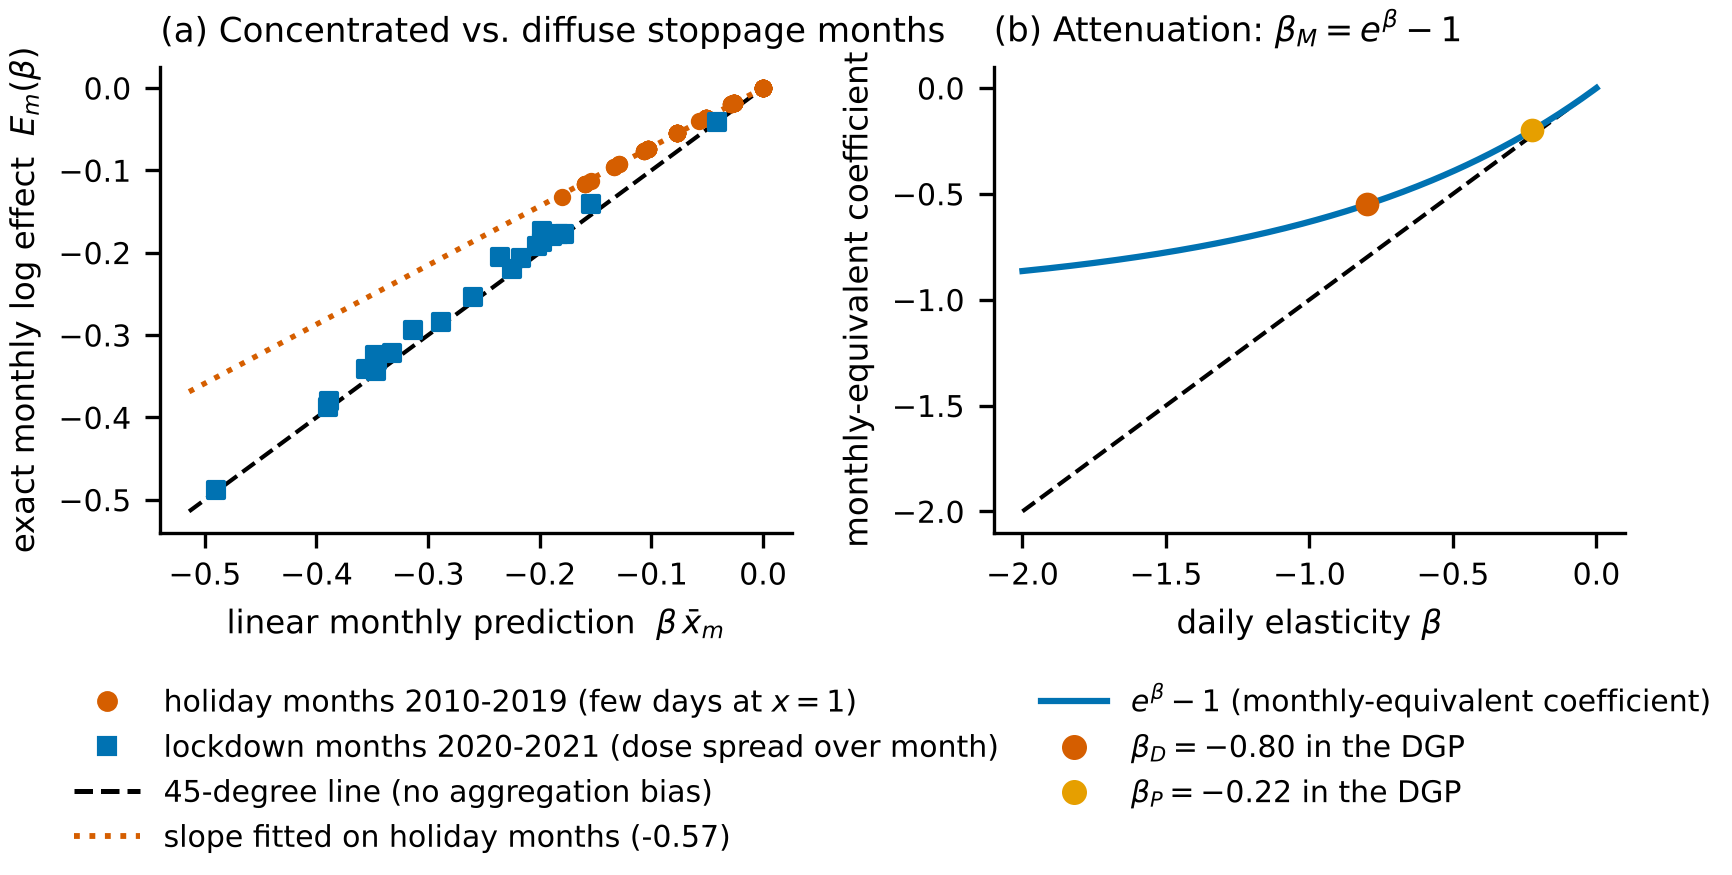
\includegraphics[width=\linewidth]{fig_jensen.png}
\caption{Aggregation bias (Proposition~\ref{prop:jensen}). (a) Exact monthly log effect against its linear approximation for the domestic channel: vermilion circles are holiday months 2010--2019, blue squares are lockdown months 2020--2021 with the S1 dose; the black dashed line is the 45-degree line and the vermilion dotted line the slope fitted on holiday months. Holiday months lie above the 45-degree line, lockdown months on it. (b) The monthly-equivalent coefficient $e^{\beta}-1$ (blue) against the daily elasticity (black dashed: identity); the vermilion and orange points mark the domestic and partner elasticities of the data-generating process.}
\label{fig:jensen}
\end{figure}

\begin{corollary}[Aggregation correction]\label{cor:ac}
For holiday shares that are small, inverting Proposition~\ref{prop:jensen}(c) gives the closed-form correction $\hat\beta_D^{AC}=\log(1+\hat\beta_M)$ for $\hat\beta_M>-1$, with delta-method variance $\operatorname{Var}(\hat\beta_D^{AC})\approx\operatorname{Var}(\hat\beta_M)/(1+\hat\beta_M)^2$. The exact minimum-distance version, $\hat\beta_D^{AC}=\arg\min_b\sum_m\{E_m(b)-\hat\beta_M\bar x_m\}^2$, uses the actual holiday composition of each month and requires only the daily regressors, not daily exports.
\end{corollary}

The correction removes the bias but inflates the variance by the factor $(1+\hat\beta_M)^{-2}$, which equals about 4.7 at $\hat\beta_M=-0.54$. Bias and variance are traded off, not eliminated.

\begin{proposition}[Identification at monthly frequency]\label{prop:ident}
In the monthly regression of $\log(Y_m/D_m)$ on calendar-month effects, a trend and $\bar x^D_m$, the Frisch--Waugh--Lovell theorem gives $\operatorname{Var}(\hat\beta_M)=\sigma_m^2/\sum_m\tilde x_m^2$, where $\tilde x_m$ is the residual of $\bar x^D_m$ after projection on the calendar-month effects and the trend. Because Songkran falls on 13--15 April every year, its contribution to $\bar x^D_m$ is absorbed by the April effect, and $\hat\beta_M$ is identified only by year-to-year variation in the number of holidays per month (in-lieu days, lunar Buddhist holidays, special holidays and the 2020 postponement). In daily data, $\beta_D$ is identified by contrasts between holidays and adjacent working days, which are nearly orthogonal to smooth seasonality.
\end{proposition}

For 2010--2019 the standard deviation of $\bar x^D_m$ is <<xraw.sd>>, but after removing calendar-month means it falls to <<xres.sd>>, roughly <<xres.days>> of a holiday day per month. The corresponding daily residual standard deviation is <<xdres.sd>>.

\begin{proposition}[Dose saturation in tree ensembles]\label{prop:tree}
Let $f$ be an ensemble of regression trees trained on data in which a feature $x$ takes only the values 0 and 1. Every split on $x$ uses a threshold $c\in(0,1)$, and with histogram binning all trees share the same threshold. Holding the other features fixed, $f$ takes only the two values $f(0)$ and $f(1)$, so $f(\lambda h)=f(1)$ for every dose $\lambda h>c$. If $x$ is continuous with training support $[0,a]$, then $f(x)=f(a)$ for $x>a$.
\end{proposition}

In LightGBM the threshold for a binary feature is placed at $10^{-35}$, which we verified in the fitted trees: any positive dose is treated as a full holiday.

\section{Simulation design}\label{sec:design}
We follow the ADEMP structure of \citet{morris2019simulation}: aims, data-generating mechanisms, estimands, methods and performance measures.

\subsection{Aims}
The study evaluates whether stoppage elasticities identified from recurring holidays transfer to lockdowns (RQ1), how accuracy depends on the dose scale and its calibration (RQ2), what monthly data lose (RQ3), whether tree ensembles can transfer (RQ4) and how the shock should be handled afterwards (RQ5). Simulation is necessary because the true elasticities, pass-through and doses are unknown in official data.

\subsection{Data-generating mechanisms}
\paragraph{Real inputs.} The holiday calendar is the observed Thai calendar from the \texttt{holidays} package \citep{pyholidays}, excluding National Children's Day, which is not a day off. Chinese-New-Year dates are taken from the Chinese calendar in the same package. Daily national stringency indices for Thailand and China come from OxCGRT \citep{hale2021oxcgrt}, and daily workplace mobility for Thailand from the Google Community Mobility Reports \citep{google2022mobility}. Figure~\ref{fig:drivers} displays these inputs.

\begin{figure}[p]
\centering
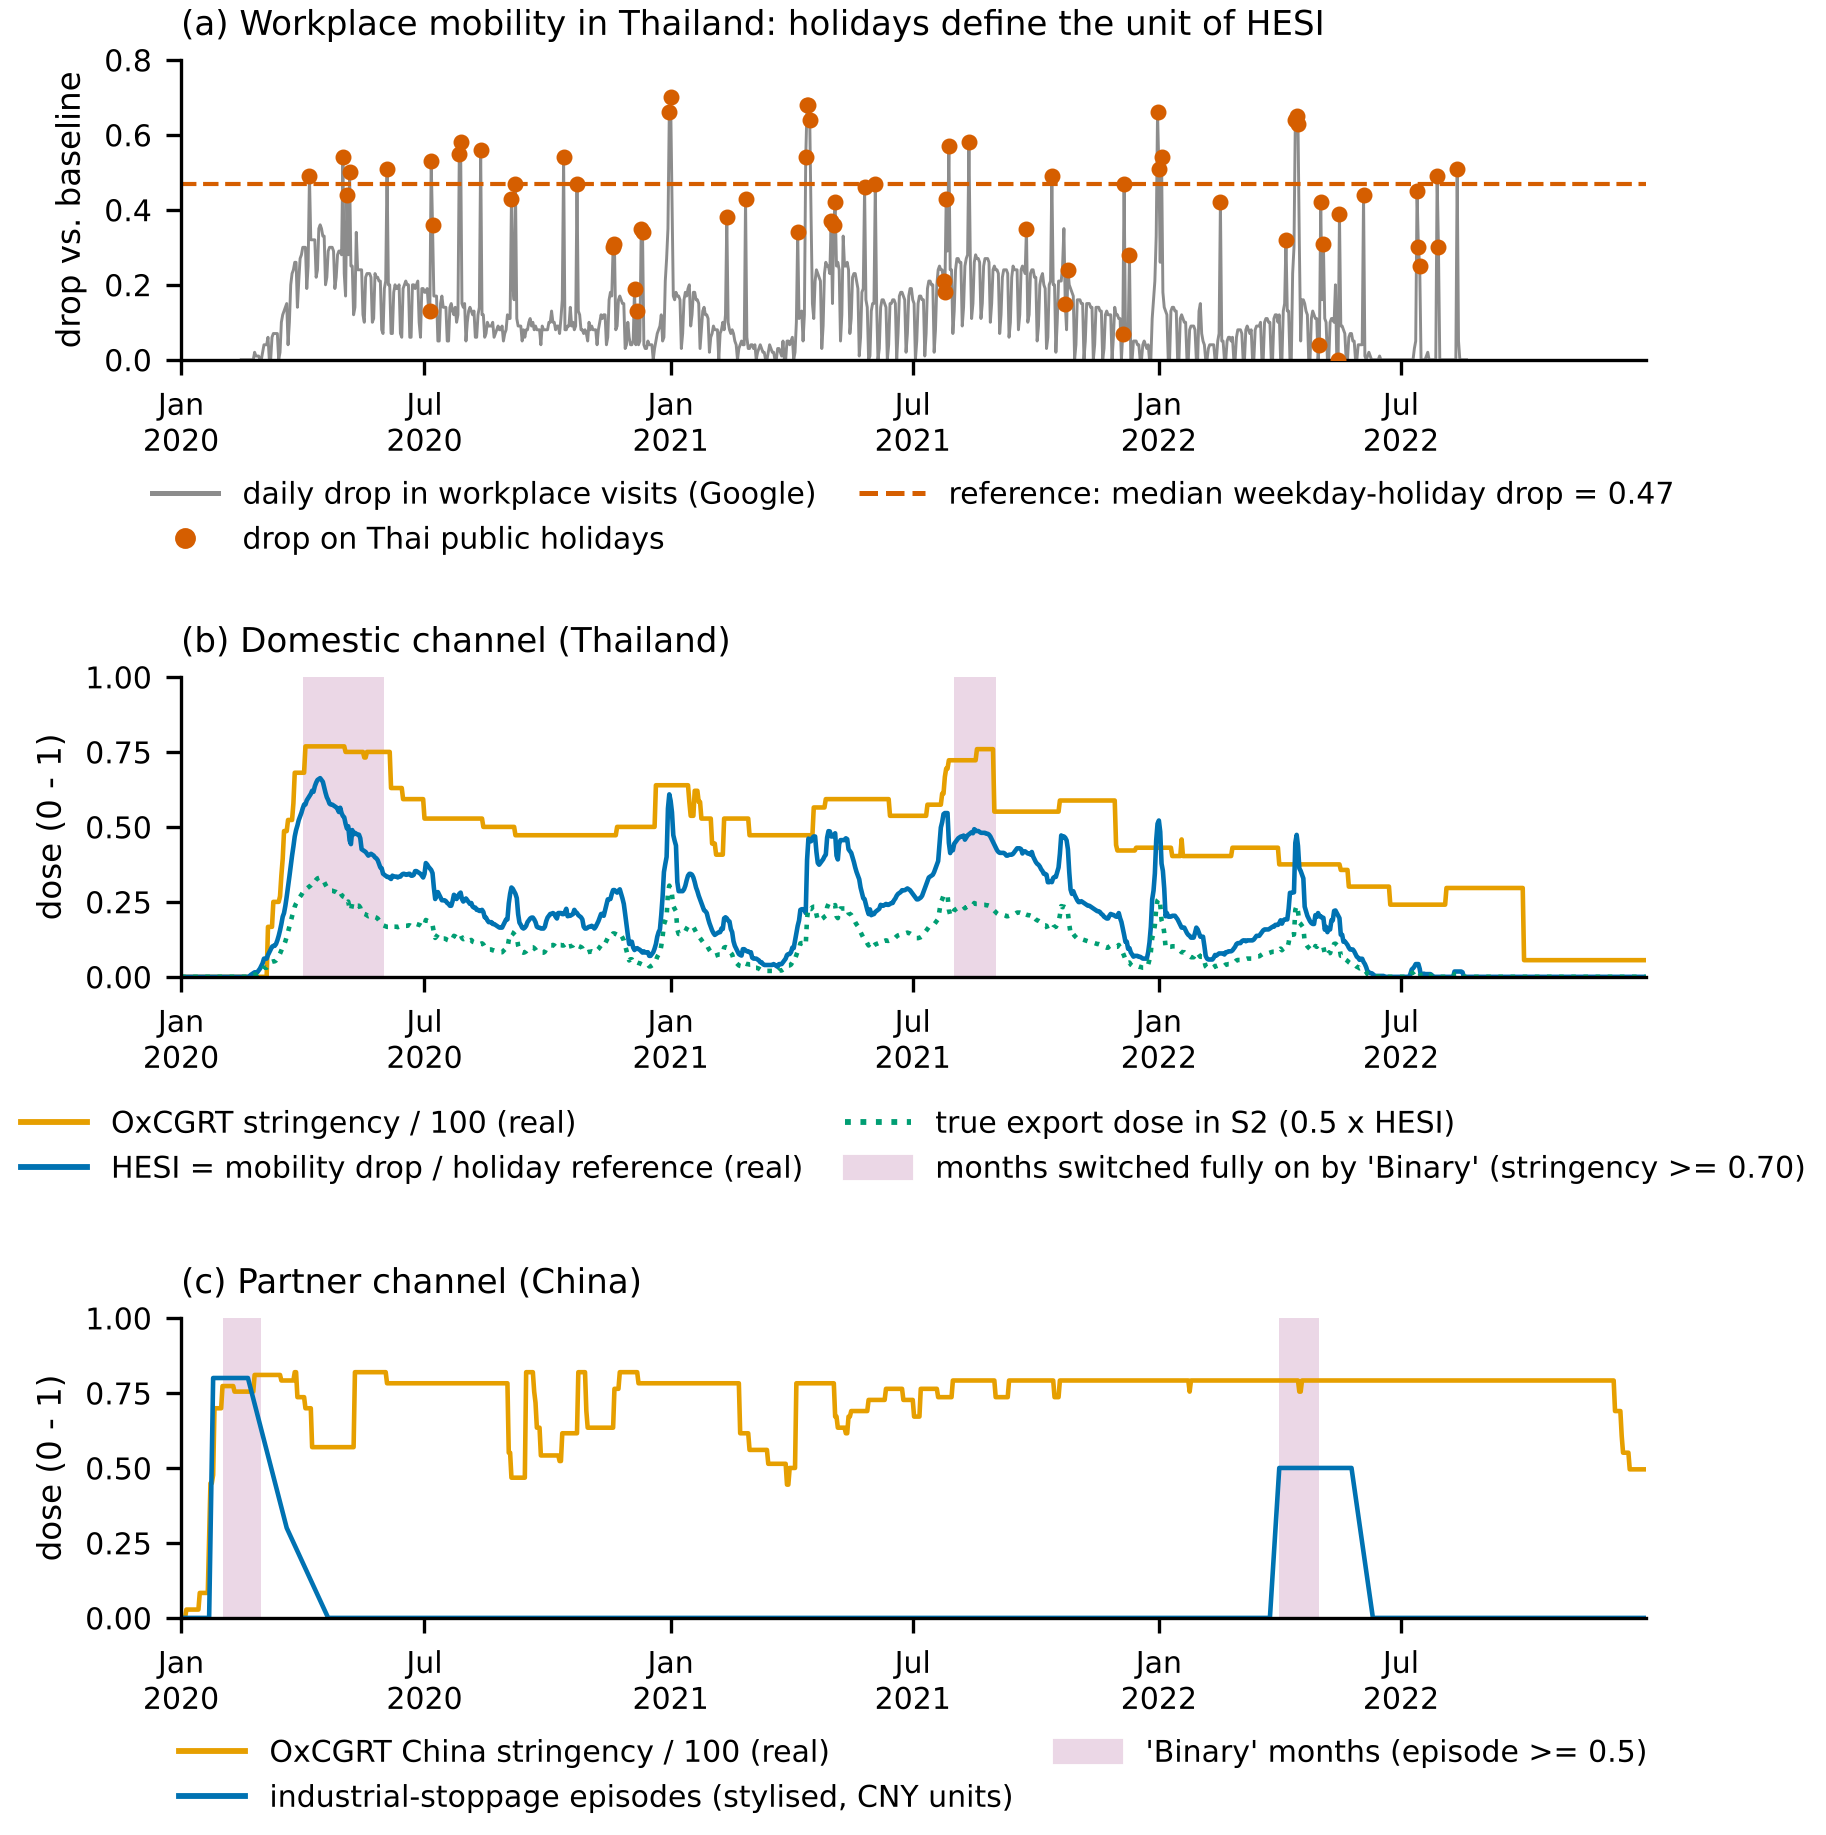
\includegraphics[width=\linewidth]{fig_drivers.png}
\caption{Real pandemic inputs. (a) Daily drop in workplace visits in Thailand (grey line) and the drop on public holidays (vermilion points); the vermilion dashed line is the median drop on weekday holidays, which defines one holiday unit of HESI. (b) Domestic channel: OxCGRT stringency (orange), HESI (blue) and the true export dose of scenario S2 (green dotted); lilac bands mark the months that the Binary variant switches fully on. (c) Partner channel: OxCGRT stringency for China (orange) stays high for three years, whereas industrial-stoppage episodes (blue) are short; lilac bands mark the Binary months.}
\label{fig:drivers}
\end{figure}

\paragraph{Data-generating process.} Daily exports from 1 January 2010 to 31 December 2024 follow~\eqref{eq:model} with the parameters in Table~\ref{tab:dgp}. The level and trend place annual exports in the range of USD 200--300 billion, the order of magnitude of Thai merchandise exports. Holidays reduce exports by 55\% ($\beta_D=\log0.45$) and each day of the Chinese-New-Year window by 20\% ($\beta_P=\log0.80$). The true pandemic doses follow~\eqref{eq:measurement} with an AR(1) proxy error $\nu_d$ (persistence 0.97, stationary standard deviation 0.15), so mobility is an imperfect proxy even in the best case.

\paragraph{Scenarios.} In \emph{S1 (ideal transfer)} the pass-through is $\kappa=1$ and there is no demand shock: Assumptions~\ref{ass:inv}--\ref{ass:add} hold and HESI is correctly scaled up to $\nu_d$. In \emph{S2 (realistic)} the pass-through is $\kappa=0.5$, so mobility overstates the stoppage two-fold, and a global demand shock that HESI cannot see lowers exports by 8\% in April--June 2020 and raises them by 7\% in 2021 before fading by mid-2022. Each replication uses the same random numbers in both scenarios (common random numbers), so differences between scenarios are not driven by noise. Figure~\ref{fig:data} shows one replication.

\paragraph{Robustness mechanisms.} \emph{R1 (heterogeneous holidays)} replaces the common holiday effect with $\log0.35=-1.05$ for festival days (Songkran and New Year) and $\log0.55=-0.60$ for ordinary holidays, with the pandemic dose measured in ordinary-holiday units. \emph{R2 (real-time dose)} replaces the centred smoothing in~\eqref{eq:hesi} with a trailing seven-day window available in real time.

\begin{table}[t]
\centering\small
\caption{Parameters of the daily data-generating process (log scale).}
\label{tab:dgp}
\begin{tabular}{p{0.28\linewidth}p{0.64\linewidth}}
\toprule
Component & Specification \\
\midrule
Level & USD 560 million per day in 2010 (about USD 200 billion per year) \\
Trend & $+10\%$/yr (2010--11), $-1\%$/yr (2012--15), $+2.5\%$/yr (2016--19), $+3\%$/yr (2020--22), $+2\%$/yr (2023--24) \\
Yearly seasonality & three Fourier harmonics, amplitude about $\pm6\%$ \\
Day of week & Monday--Friday $+0.02$ to $+0.04$; Saturday $-0.30$; Sunday $-0.55$ \\
Holiday elasticity $\beta_D$ & $\log 0.45=-0.80$ per holiday-equivalent day \\
Partner elasticity $\beta_P$ & $\log 0.80=-0.22$ per day in the Chinese-New-Year window \\
Pandemic doses & domestic $\kappa h_d(1+\nu_d)$; partner $p_d(1+\nu'_d)$; $\nu,\nu'$ AR(1), $\rho=0.97$, s.d.\ 0.15 \\
Disturbances & daily AR(1) $\rho=0.985$ (stationary s.d.\ 0.046); monthly AR(1) $\rho=0.85$ (innovation s.d.\ 0.015); i.i.d.\ s.d.\ 0.12 \\
S1 & $\kappa=1$, no demand shock \\
S2 & $\kappa=0.5$; demand $-8\%$ in Apr--Jun 2020, $+7\%$ in 2021, zero after mid-2022 \\
\bottomrule
\end{tabular}
\end{table}

\begin{figure}[t]
\centering
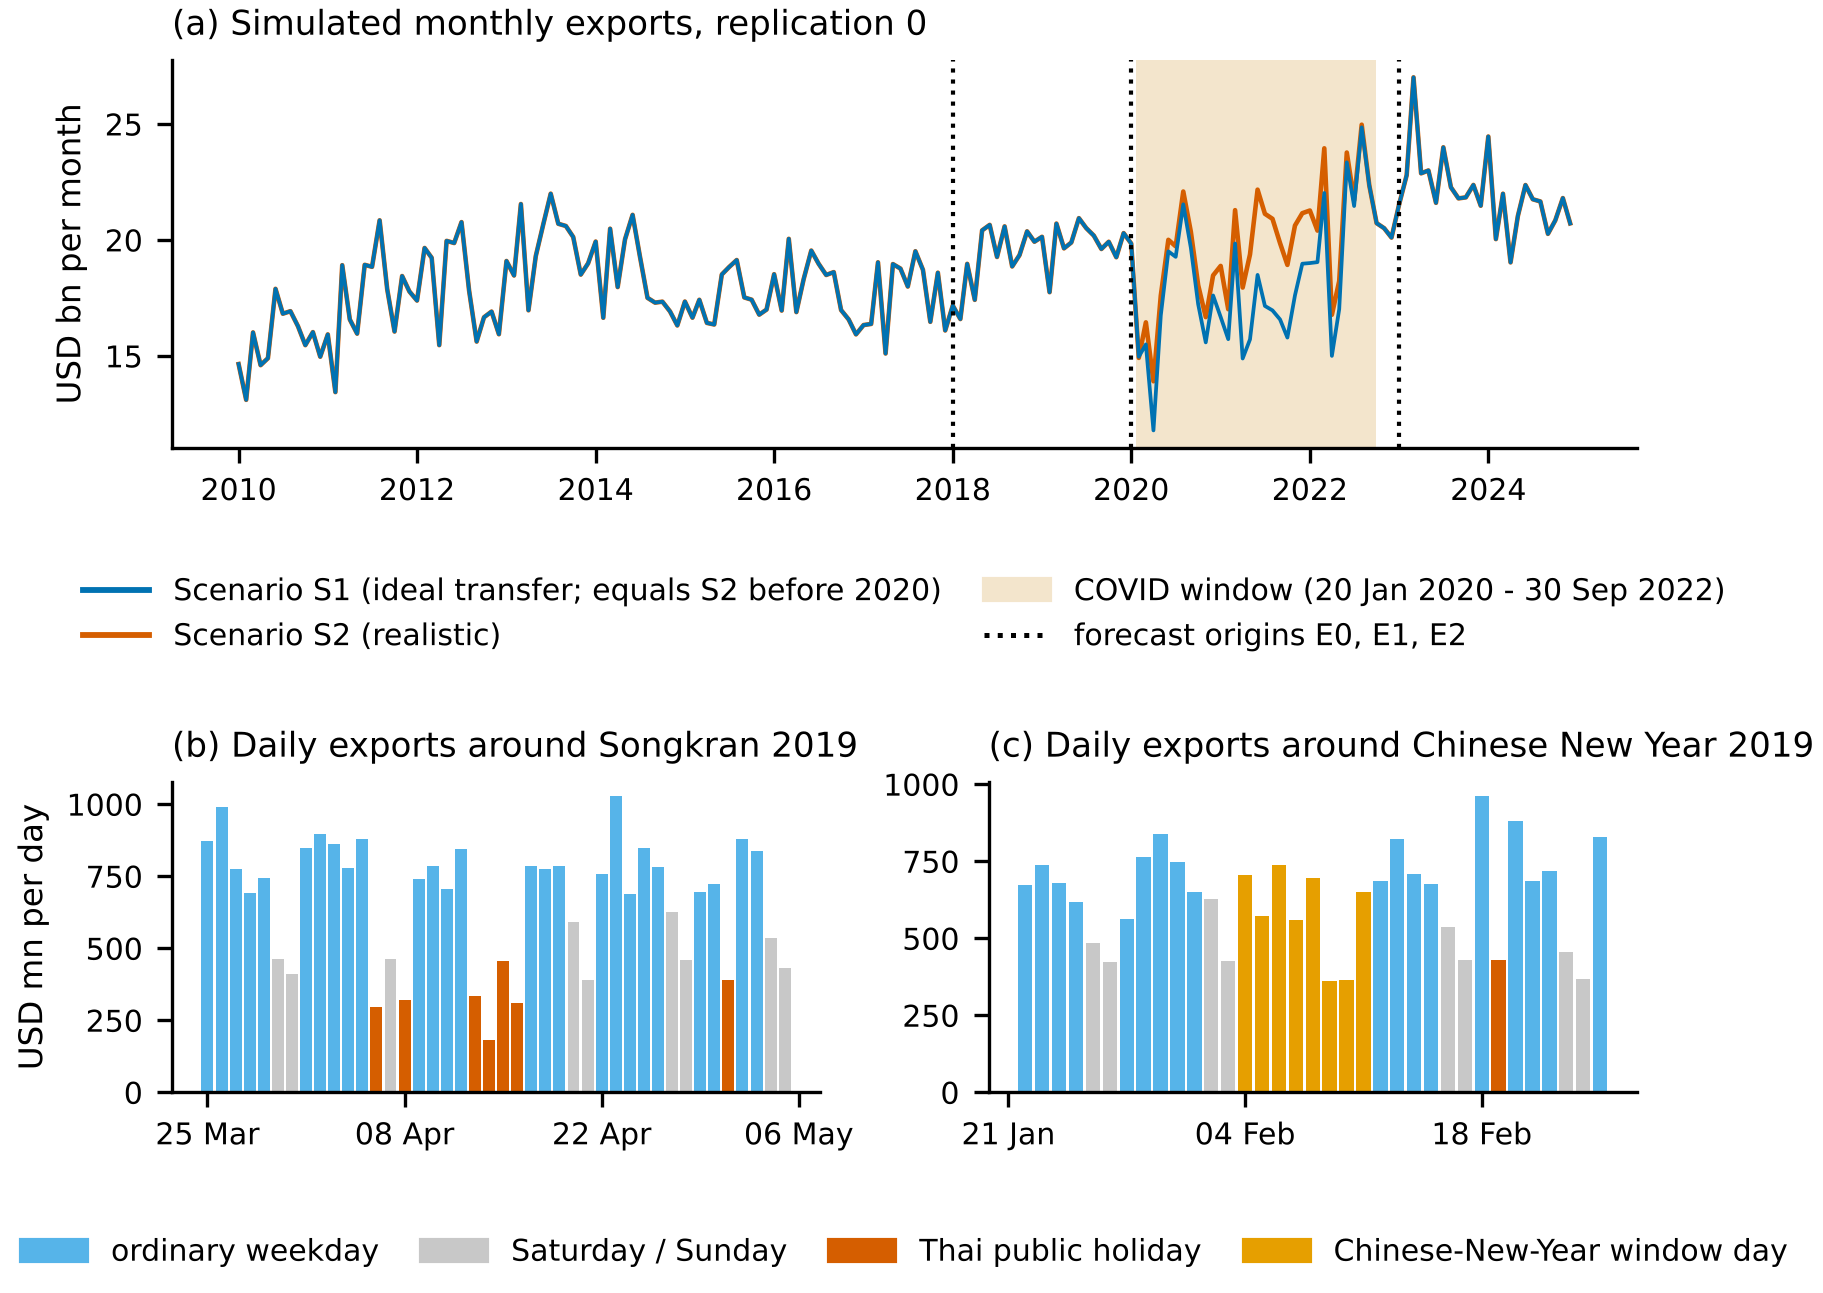
\includegraphics[width=\linewidth]{fig_data.png}
\caption{Simulated data, replication 0. (a) Monthly totals in S1 (blue) and S2 (vermilion), which coincide before 2020 because they share the same random numbers; the tan band is the pandemic window and the dotted black lines are the forecast origins of experiments E0, E1 and E2. (b)--(c) Daily values around Songkran and the Chinese New Year 2019, coloured by day type: sky blue for ordinary weekdays, light grey for weekends, vermilion for Thai public holidays and orange for days in the Chinese-New-Year window.}
\label{fig:data}
\end{figure}

\subsection{Estimands}
The primary estimand is the monthly export total in each test window, evaluated by MAPE and by the mean absolute scaled error (MASE) of \citet{hyndman2006another}, scaled by the in-sample seasonal-naive error. Secondary estimands are the elasticities $\beta_D$ and $\beta_P$ (bias, standard deviation and root mean squared error across replications) and the calibrated dose $\hat\lambda$ relative to $\kappa$.

\subsection{Methods}
Table~\ref{tab:models} lists the forecasting methods and the dose variants. All hyperparameters are fixed in advance; nothing is tuned on test data.

\begin{table}[t]
\centering\small
\caption{Methods and dose variants.}
\label{tab:models}
\begin{tabular}{p{0.30\linewidth}p{0.62\linewidth}}
\toprule
Method & Specification \\
\midrule
Seasonal naive & value of the same month in the last training year \\
Prophet daily (vanilla) & Prophet on $\log y_d$ without calendar regressors, summed to months \\
Prophet daily (P-D) & Prophet on $\log y_d$ with shared regressors $x^D_d$, $x^P_d$ \\
Prophet monthly (P-M) & Prophet on $\log(Y_m/D_m)$ with $\bar x^D_m$, $\bar x^P_m$, $\mathrm{WK}_m$ (Fourier order 5, 15 changepoints) \\
P-M + AC & P-M with the aggregation correction of Corollary~\ref{cor:ac} \\
SARIMAX & airline model $(0,1,1)(0,1,1)_{12}$ on $\log(Y_m/D_m)$ with the P-M regressors \citep{box2015time} \\
LightGBM daily / monthly & OLS log-linear trend plus LightGBM on the detrended residual; daily features: day of week, day of year, $x^D_d$, $x^P_d$; monthly features: month, $\bar x^D_m$, $\bar x^P_m$, $\mathrm{WK}_m$ \\
\midrule
\multicolumn{2}{l}{\textit{Dose variants in the shock period (E1)}} \\
Off & holidays only, no pandemic dose \\
Binary whole-month switch & $x^D=1$ on every day of months with mean stringency $\ge0.70$; $x^P=1$ in months with episode index $\ge0.5$ \\
Raw stringency & OxCGRT stringency/100 for Thailand and China used as doses \\
HESI ($\lambda=1$) & mobility-based HESI for Thailand; episode index for China \\
HESI-cal ($\hat\lambda$) & $\hat\lambda\in\{0,0.05,\dots,3\}$ minimising squared log errors in March--April 2020; evaluated May 2020--December 2021 \\
Oracle ($\kappa$ known) & $\lambda=\kappa$; the proxy error $\nu_d$ and the demand shock remain unknown \\
\midrule
\multicolumn{2}{l}{\textit{Treatments of the pandemic in the training sample (E2)}} \\
COVID ignored & holiday regressors only \\
Mask COVID window & observations from 20 January 2020 to 30 September 2022 removed \\
Separate COVID regressors & HESI and episode index enter with their own coefficients \\
Binary, raw stringency, HESI & the corresponding shared regressors enter the training sample \\
\bottomrule
\end{tabular}
\end{table}

\subsection{Experiments}
\textbf{E0 (normal period)}: training to December 2017, forecasts for January 2018--December 2019. \textbf{E1 (shock period)}: training to December 2019, forecasts for January 2020--December 2021. The doses observed during the forecast window are supplied to the models, so E1 evaluates \emph{scenario-conditional} forecasts (equivalently, nowcasts conditional on observed mobility), not ex-ante forecasts. Accuracy is reported over the full 24 months and over May 2020--December 2021, the window that follows the calibration months of HESI-cal. \textbf{E2 (aftermath)}: training to December 2022, including the pandemic, and forecasts for January 2023--December 2024 with no pandemic doses.

\subsection{Performance measures and inference}
For each method we report the mean across <<nseeds>> replications and its Monte Carlo standard error. Because all methods are applied to the same replications, comparisons are paired: for each comparison we report the mean paired difference in MAPE with a 95\% $t$-interval, the share of replications in which the first method is more accurate, and the Wilcoxon signed-rank test \citep{wilcoxon1945individual}, with Holm's correction across the family of comparisons. In this setting the replication, not the month, is the unit of inference, so we do not apply Diebold--Mariano tests \citep{diebold1995comparing, harvey1997testing} within replications; they are part of the protocol for official data (Section~\ref{sec:protocol}).

\section{Results}\label{sec:results}
\subsection{Transfer during the shock (E1)}
Table~\ref{tab:e1} reports the accuracy of all methods in the shock period, and Figure~\ref{fig:paths} shows the forecast paths of one replication. In S1, daily Prophet with HESI reduces the MAPE from <<e1.s1.pd.off.w24>>\% without a dose to <<e1.s1.pd.hesi.w24>>\%, and it is more accurate than the no-dose forecast in <<win.s1.hesi.off>>\% of replications. The model never observes a pandemic day: the entire improvement comes from the elasticity identified on holidays before 2020. This answers RQ1 affirmatively under the assumptions of S1.

The whole-month switch reduces the MAPE only to <<e1.s1.pd.binary.w24>>\%. Consistent with Proposition~\ref{prop:transfer}(c), it overshoots in the three months that it switches on, where it predicts a 55\% loss for the whole month, and it leaves the remaining months of partial stoppage unadjusted. Raw stringency raises the MAPE to <<e1.s1.pd.stringency.w24>>\%, mainly because China's stringency index assigns a dose of 0.6--0.8 to a partner that was largely operating.

In S2, where mobility overstates the stoppage two-fold and a demand shock is present, HESI with $\lambda=1$ improves on the no-dose forecast on average (<<e1.s2.pd.hesi.w24>>\% against <<e1.s2.pd.off.w24>>\%) but not consistently: it wins in <<pw.c1.s2>>\% of replications, and the difference is not significant after Holm's correction (adjusted $p$ = <<ph.c1.s2>>). It also falls short of the oracle (<<e1.s2.pd.oracle.w24>>\%). Calibrating the dose on March--April 2020 lowers the MAPE over May 2020--December 2021 to <<e1.s2.pd.cal.w20>>\%, against <<e1.s2.pd.off.w20>>\% without a dose and <<e1.s2.pd.oracle.w20>>\% for the oracle. The calibrated dose is significantly better than the uncalibrated one (adjusted $p$ = <<ph.c5.s2>>), whereas its advantage over the no-dose forecast is significant only before adjustment (adjusted $p$ = <<ph.c4.s2>>). Figure~\ref{fig:dist} shows the corresponding distributions across replications.

One result requires care. In S2 the monthly model with $\lambda=1$ is more accurate than the daily model (<<e1.s2.pm.hesi.w24>>\% against <<e1.s2.pd.hesi.w24>>\%). This is not an advantage of monthly data but a cancellation of two errors: the attenuated monthly coefficient (Proposition~\ref{prop:jensen}) offsets the two-fold overstatement of the dose. When the dose is correctly scaled (S1), the ranking reverses (<<e1.s1.pd.hesi.w24>>\% against <<e1.s1.pm.hesi.w24>>\%).

\begin{figure}[t]
\centering
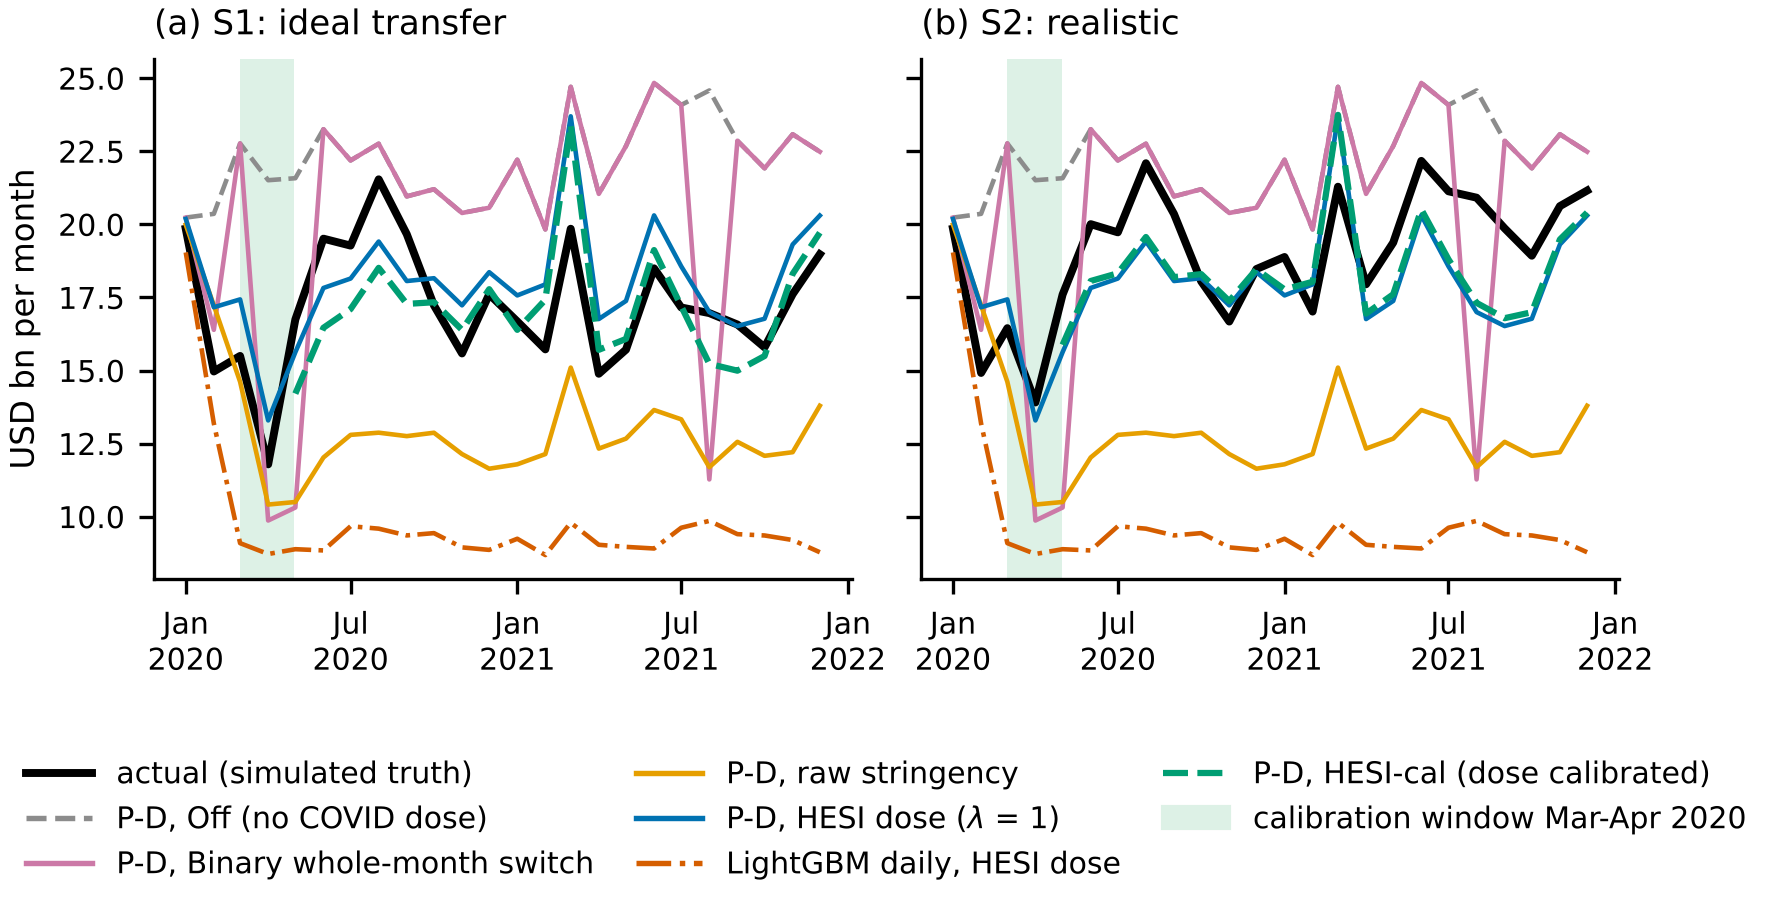
\includegraphics[width=\linewidth]{fig_e1_paths.png}
\caption{Forecasts for the shock period from December 2019 (replication 0). Black: actual simulated totals. Grey dashed: P-D without a dose. Lilac: P-D with the Binary whole-month switch. Orange: P-D with raw stringency. Blue: P-D with HESI ($\lambda=1$). Green dashed: P-D with the calibrated dose, shown from May 2020. Vermilion dash-dot: LightGBM daily with HESI. The mint band marks the calibration window, March--April 2020.}
\label{fig:paths}
\end{figure}

\begin{figure}[t]
\centering
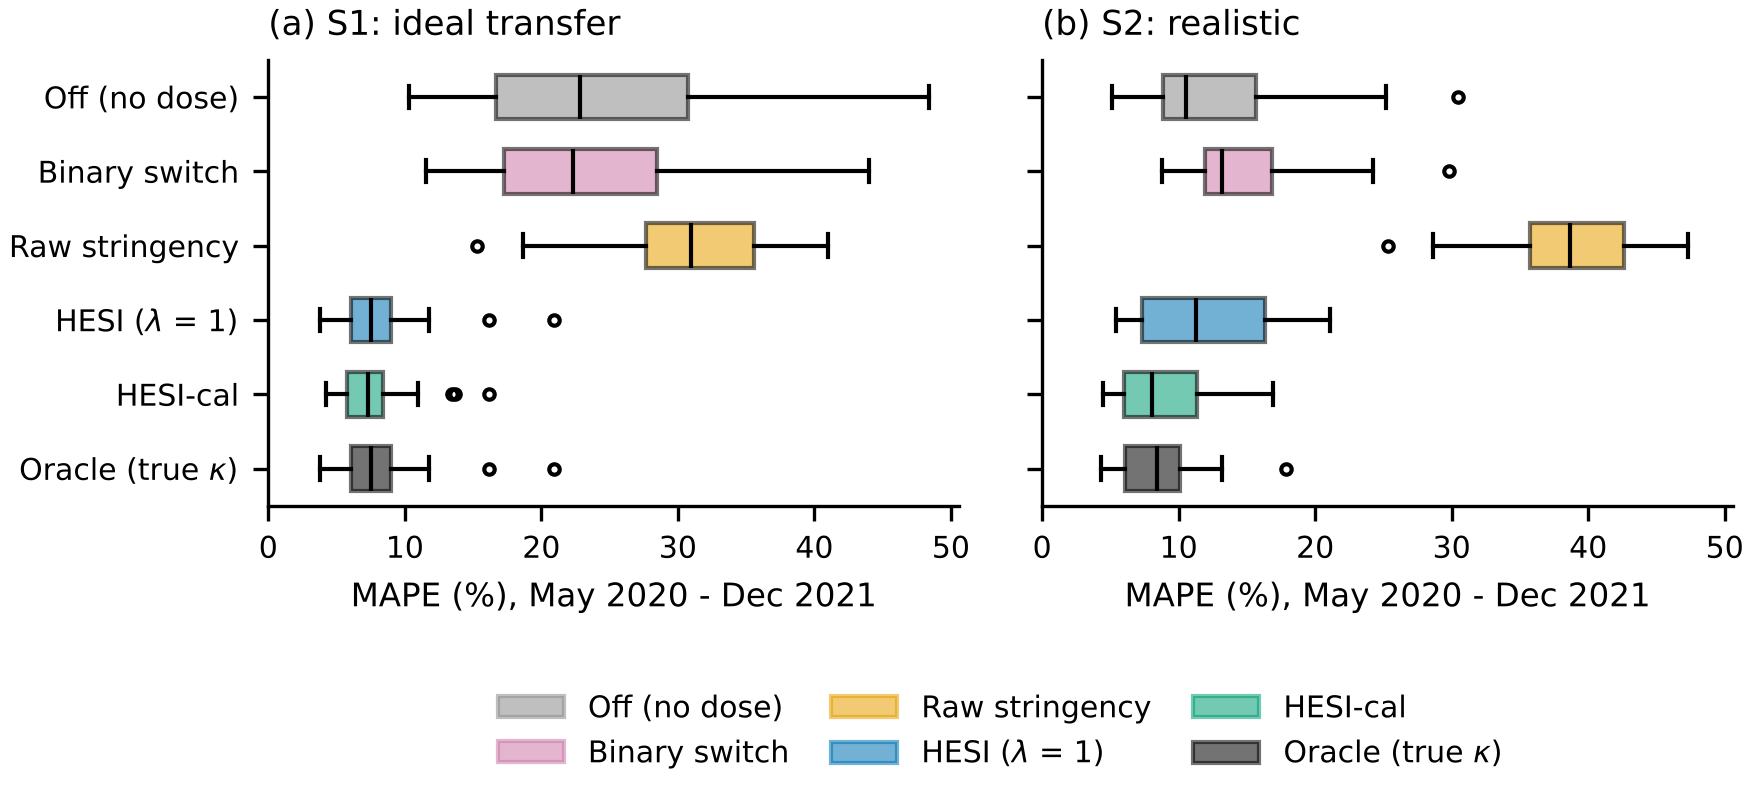
\includegraphics[width=\linewidth]{fig_e1_dist.png}
\caption{Distribution of the MAPE of daily Prophet across <<nseeds>> replications, May 2020--December 2021, by dose variant. Box colours: grey for no dose, lilac for the Binary switch, orange for raw stringency, blue for HESI with $\lambda=1$, green for the calibrated dose and dark grey for the oracle. Boxes show the interquartile range, black lines the median, whiskers 1.5 times the interquartile range and circles the remaining replications.}
\label{fig:dist}
\end{figure}

\begin{table}[!tb]
\centering
\caption{Shock period (E1): MAPE (\%), mean over <<nseeds>> replications with Monte Carlo standard errors in parentheses. Bold: lowest value in each column excluding the oracle. ``Jan--Dec'' denotes January 2020--December 2021; ``May--Dec'' denotes May 2020--December 2021.}
\label{tab:e1}
\footnotesize
\begin{tabular}{llcccc}
\toprule
 & & \multicolumn{2}{c}{S1: ideal transfer} & \multicolumn{2}{c}{S2: realistic} \\
\cmidrule(lr){3-4}\cmidrule(lr){5-6}
Method & Dose variant & Jan--Dec & May--Dec & Jan--Dec & May--Dec \\
\midrule
%%TAB_E1%%
\bottomrule
\end{tabular}
\end{table}

\subsection{Dose sensitivity and real-time calibration}
Figure~\ref{fig:lambda} traces the MAPE as a function of the dose multiplier $\lambda$. For daily Prophet the curve is U-shaped with its minimum at $\lambda=<<lamopt.s1.pd>>$ in S1 (true $\kappa=1$) and at $\lambda=<<lamopt.s2.pd>>$ in S2 (true $\kappa=0.5$), as Proposition~\ref{prop:transfer} predicts. For the monthly models the minimum shifts to the right, to <<lamopt.s1.pm>> for Prophet and <<lamopt.s1.sx>> for SARIMAX in S1: an attenuated elasticity requires an inflated dose. The aggregation correction moves the minimum back to <<lamopt.s1.pmac>> in S1 and <<lamopt.s2.pmac>> in S2, but its larger variance keeps its minimum error above that of the daily model.

Table~\ref{tab:lamhat} reports the doses selected by real-time calibration. Daily Prophet selects $\hat\lambda=<<lam.s1.pd>>$ in S1 and $<<lam.s2.pd>>$ in S2. The upward deviation in S2 is the absorption effect of Proposition~\ref{prop:transfer}(b): evaluating~\eqref{eq:lamstar} with the true demand path over the non-holiday days of March--April 2020 gives $\lambda^{*}=<<lamstar.cal>>$, close to the mean calibrated value. Calibration on exports alone cannot distinguish stoppage from a coincident demand collapse.

\begin{figure}[t]
\centering
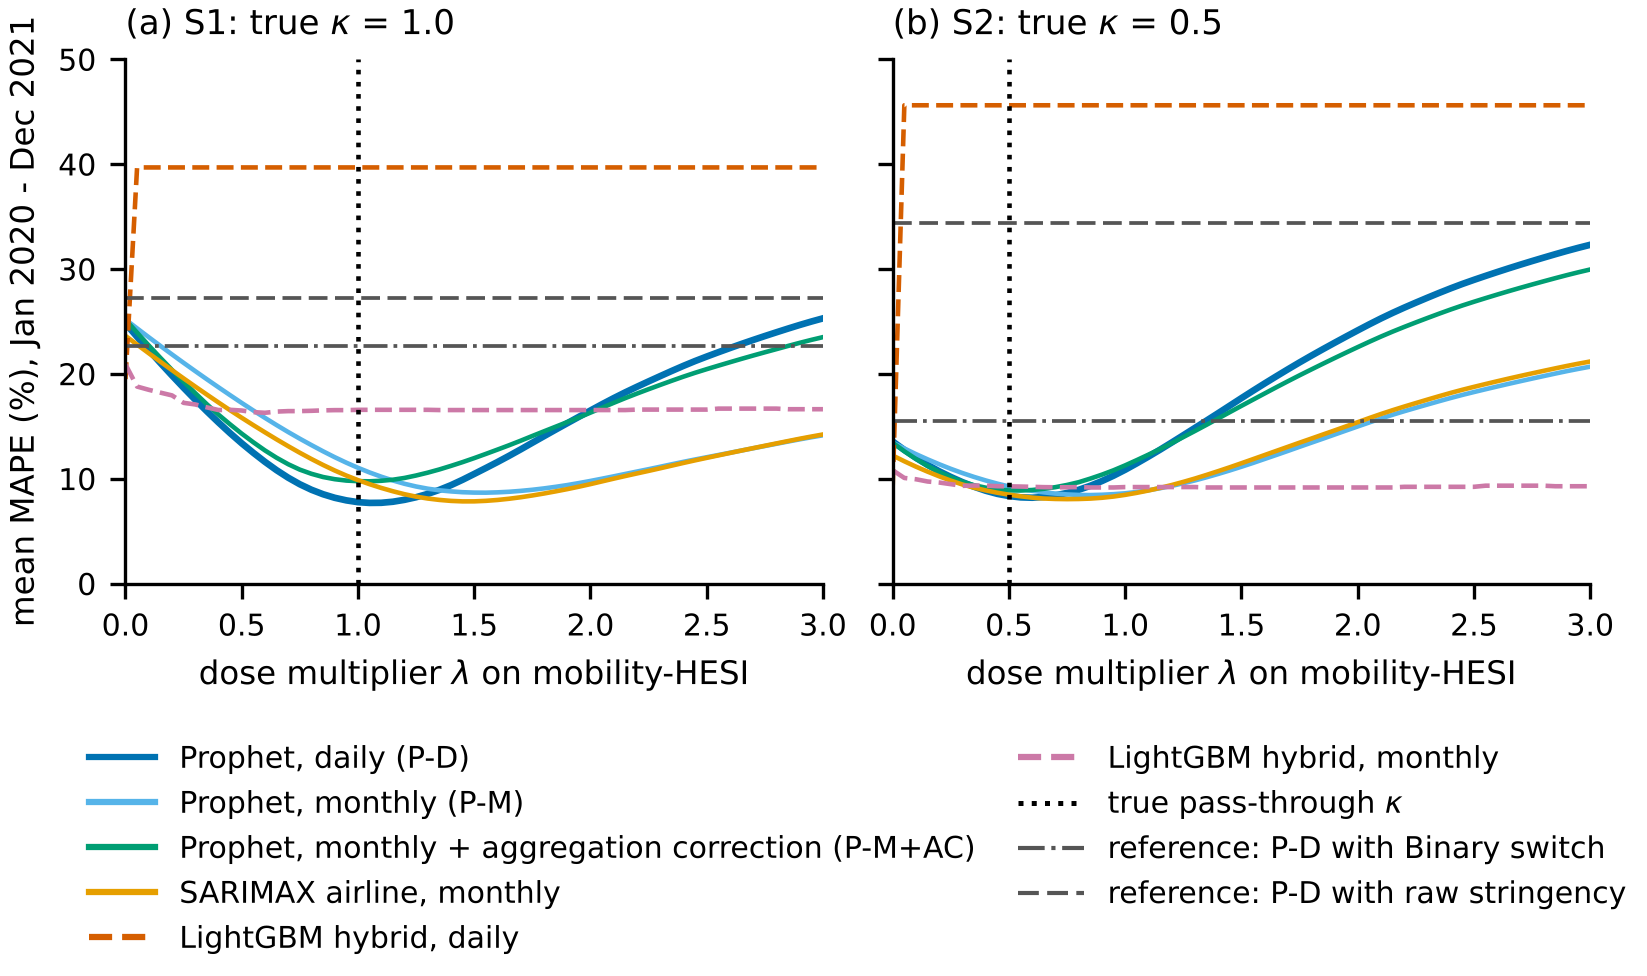
\includegraphics[width=\linewidth]{fig_lambda.png}
\caption{Mean MAPE over January 2020--December 2021 as a function of the dose multiplier $\lambda$ applied to HESI. Line colours identify methods: blue for daily Prophet, sky blue for monthly Prophet, green for monthly Prophet with aggregation correction, orange for SARIMAX, vermilion dashed for daily LightGBM and lilac dashed for monthly LightGBM. The black dotted vertical line is the true pass-through $\kappa$; the grey dash-dot and dashed horizontal lines are daily Prophet with the Binary switch and with raw stringency.}
\label{fig:lambda}
\end{figure}

\begin{table}[t]
\centering\small
\caption{Calibrated dose $\hat\lambda$ selected on March--April 2020 (mean and standard deviation across replications). The true pass-through is $\kappa=1$ in S1 and $\kappa=0.5$ in S2; the last row reports the optimal dose implied by Proposition~\ref{prop:transfer}(b) for the calibration window.}
\label{tab:lamhat}
\begin{tabular}{lcccc}
\toprule
 & \multicolumn{2}{c}{S1} & \multicolumn{2}{c}{S2} \\
\cmidrule(lr){2-3}\cmidrule(lr){4-5}
Method & Mean & S.D. & Mean & S.D. \\
\midrule
%%TAB_LAMHAT%%
\bottomrule
\end{tabular}
\end{table}

\subsection{What monthly data lose: aggregation and identification}
Figure~\ref{fig:beta} and Table~\ref{tab:beta} compare the elasticities estimated from the pre-pandemic sample with their true values and with the predictions of Section~\ref{sec:theory}. Daily Prophet recovers $\beta_D$ almost exactly ($<<bD.pd>>$, standard deviation $<<bDsd.pd>>$). Monthly Prophet and SARIMAX both yield $<<bD.pm>>$, close to the aggregation-implied $<<bD.implied>>$ and the closed form $<<bM.closed>>$: the attenuation is explained by Proposition~\ref{prop:jensen}. Their standard deviations, $<<bDsd.pm>>$ and $<<bDsd.sx>>$, are more than ten times that of the daily estimate, as Proposition~\ref{prop:ident} implies. The aggregation correction raises the mean to $<<bD.pmac>>$ and the standard deviation to $<<bDsd.pmac>>$; the closed form of Corollary~\ref{cor:ac} predicts $<<ac.closed>>$ and $<<ac.deltasd>>$. For the partner channel, the elasticity is small and the Chinese New Year moves between January and February, so monthly estimation is nearly unbiased ($<<bP.pm>>$ against $<<bP.true>>$; closed form $<<bPM.closed>>$) but noisy (standard deviation $<<bPsd.pm>>$ against $<<bPsd.pd>>$). These results answer RQ3: monthly data lose precision through identification and accuracy through aggregation; the correction recovers the latter but not the former.

\begin{figure}[t]
\centering
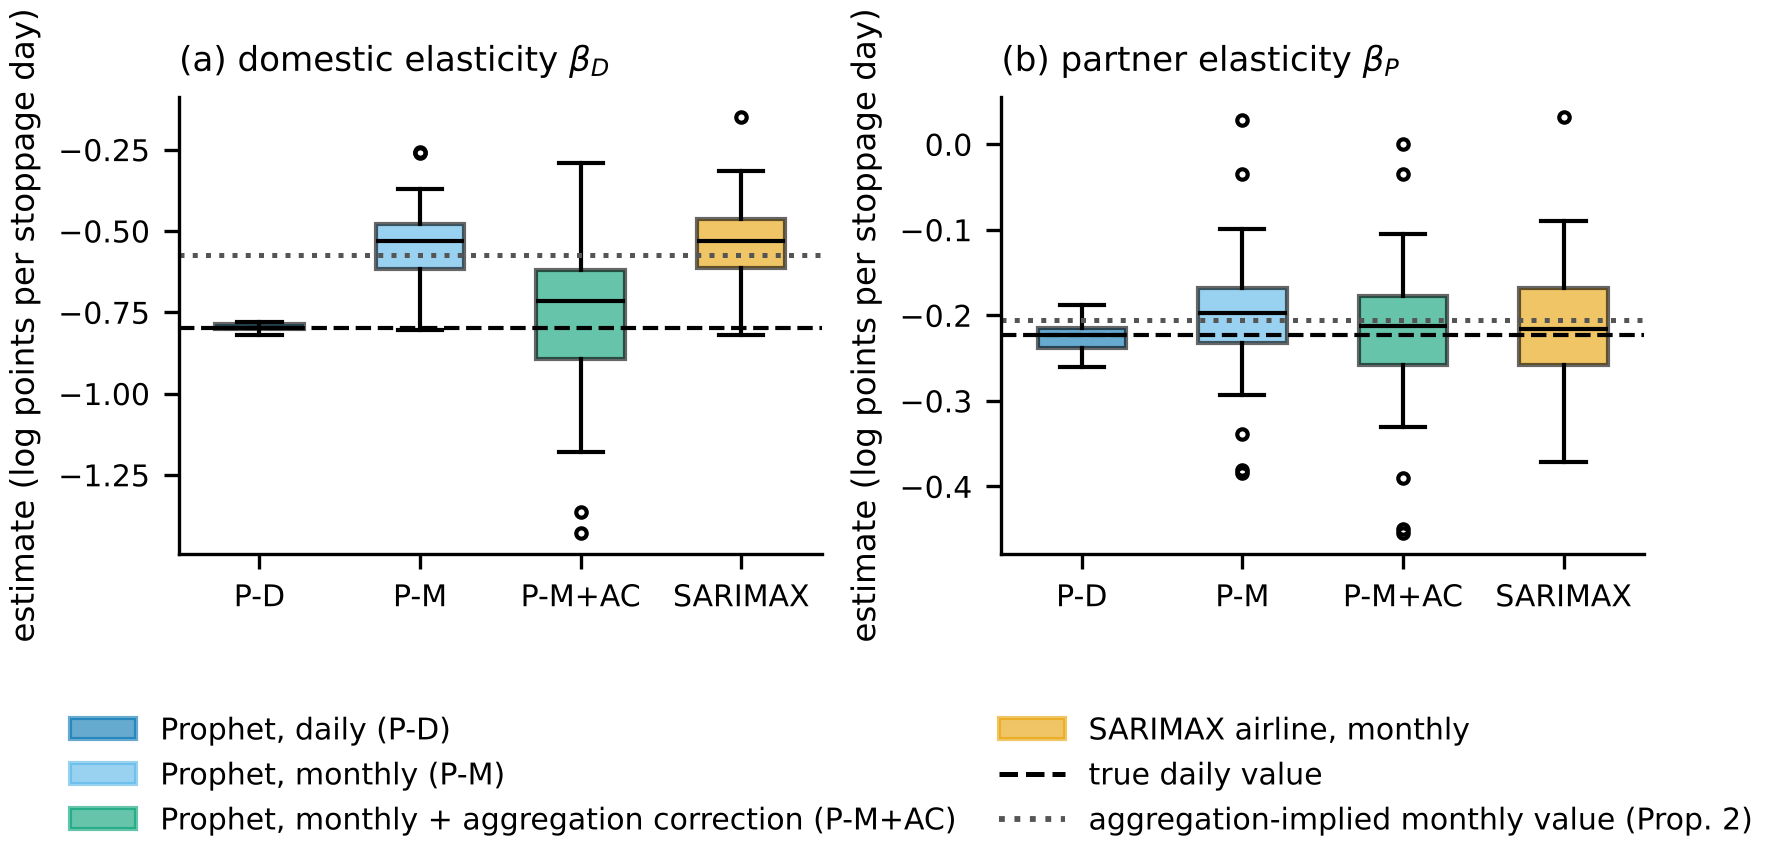
\includegraphics[width=\linewidth]{fig_beta.png}
\caption{Elasticities estimated from data up to December 2019 across <<nseeds>> replications. Box colours identify estimators: blue for daily Prophet, sky blue for monthly Prophet, green for monthly Prophet with aggregation correction and orange for SARIMAX. The black dashed line is the true daily value; the grey dotted line is the monthly value implied by exact aggregation (Proposition~\ref{prop:jensen}).}
\label{fig:beta}
\end{figure}

\begin{table}[t]
\centering\small
\caption{Estimated elasticities (E1 fits, data to December 2019): mean, standard deviation and root mean squared error with respect to the true daily value, together with theoretical benchmarks.}
\label{tab:beta}
\begin{tabular}{lcccccc}
\toprule
 & \multicolumn{3}{c}{Domestic $\beta_D$} & \multicolumn{3}{c}{Partner $\beta_P$} \\
\cmidrule(lr){2-4}\cmidrule(lr){5-7}
Estimator & Mean & S.D. & RMSE & Mean & S.D. & RMSE \\
\midrule
%%TAB_BETA%%
\bottomrule
\end{tabular}
\end{table}

\subsection{Tree ensembles saturate}
Daily LightGBM observes the stoppage regressor only at 0 and 1 before 2020 and splits it at $10^{-35}$ in every tree. Any positive dose is therefore treated as a full holiday, and the MAPE rises to <<e1.s1.ld.hesi.w24>>\% in S1 and <<e1.s2.ld.hesi.w24>>\% in S2; real-time calibration correspondingly selects a dose at or near zero (mean <<lam.s1.ld>>). Monthly LightGBM observes monthly holiday shares of at most about 0.2, whereas lockdown months reach 0.6; it predicts the effect of the most holiday-intensive month it has seen and improves the MAPE only from <<e1.s1.lm.off.w24>>\% to <<e1.s1.lm.hesi.w24>>\% in S1. These outcomes follow from Proposition~\ref{prop:tree} and do not depend on tuning, which answers RQ4.

\subsection{Robustness: heterogeneous holidays and real-time doses}\label{sec:robust}
Table~\ref{tab:robust} reports the robustness experiments. Under R1, the one-tier specification pools festival and ordinary holidays and estimates $<<r1.b1>>$, between the ordinary-holiday value ($<<r1.trueO>>$) and the festival value ($<<r1.trueF>>$). Because the dose is measured in ordinary-holiday units, the pooled elasticity acts as a dose multiplier of about <<r1.mult>>. The two-tier specification, with a separate festival indicator and the dose carried by the ordinary-holiday regressor, recovers both elasticities ($<<r1.bO>>$ and $<<r1.bF>>$). The accuracy gain is negligible in S1 (<<r1.s1.two.hesi>>\% against <<r1.s1.one.hesi>>\%), where the error curve is flat near its minimum, and larger in S2 (<<r1.s2.two.hesi>>\% against <<r1.s2.one.hesi>>\%), where the pooled elasticity compounds the overstated dose. Under R2, replacing the centred smoothing with a trailing window available in real time changes the MAPE of daily Prophet from <<r2.s1.hc>>\% to <<r2.s1.ht>>\% in S1 and from <<r2.s2.hc>>\% to <<r2.s2.ht>>\% in S2, so the results in Table~\ref{tab:e1} do not rely on future mobility data within the smoothing window.

\begin{table}[t]
\centering\small
\caption{Robustness experiments (E1, daily Prophet, <<nseeds>> replications): MAPE (\%) over January 2020--December 2021 with Monte Carlo standard errors, and estimated elasticities.}
\label{tab:robust}
\begin{tabular}{llcc}
\toprule
Specification & Dose variant & S1 & S2 \\
\midrule
%%TAB_ROBUST%%
\bottomrule
\end{tabular}
\end{table}

\subsection{Forecasting after the shock (E2)}
Table~\ref{tab:e2} and Figure~\ref{fig:e2} report forecasts for 2023--2024 from models trained through the pandemic. Ignoring the pandemic gives a daily-Prophet MAPE of <<e2.s1.pd.cal>>\% in S1 and <<e2.s2.pd.cal>>\% in S2. Including HESI in the training sample lowers it to <<e2.s1.pd.hesi>>\% and <<e2.s2.pd.hesi>>\%, and masking the pandemic window lowers it to <<e2.s1.pd.mask>>\% and <<e2.s2.pd.mask>>\%. Masking is as accurate as HESI in S1 and clearly more accurate in S2, where the overstated dose and the unmodelled rebound leak into the trend. SARIMAX, which adapts its level to the most recent observations, has the lowest mean MAPE in both scenarios (<<e2.s1.sx.hesi>>\% and <<e2.s2.sx.hesi>>\%), although its advantage over masked daily Prophet is not statistically significant (adjusted $p$ = <<ph.c12.s1>> and <<ph.c12.s2>>). Raw stringency is harmful (<<e2.s1.pd.stringency>>\% and <<e2.s2.pd.stringency>>\%): the Chinese index stays high throughout the pandemic part of the training sample and drops to zero in the forecast period, so the model forecasts an immediate jump in exports. For RQ5, the evidence favours simple treatments---masking, or models that adapt their level---over structural treatments of the shock once it has ended.

\begin{table}[t]
\centering
\caption{Aftermath (E2, January 2023--December 2024): MAPE (\%) with Monte Carlo standard errors and mean MASE. Bold: lowest MAPE in each scenario.}
\label{tab:e2}
\footnotesize
\begin{tabular}{llcccc}
\toprule
 & & \multicolumn{2}{c}{S1} & \multicolumn{2}{c}{S2} \\
\cmidrule(lr){3-4}\cmidrule(lr){5-6}
Method & Treatment of the pandemic & MAPE & MASE & MAPE & MASE \\
\midrule
%%TAB_E2%%
\bottomrule
\end{tabular}
\end{table}

\begin{figure}[t]
\centering
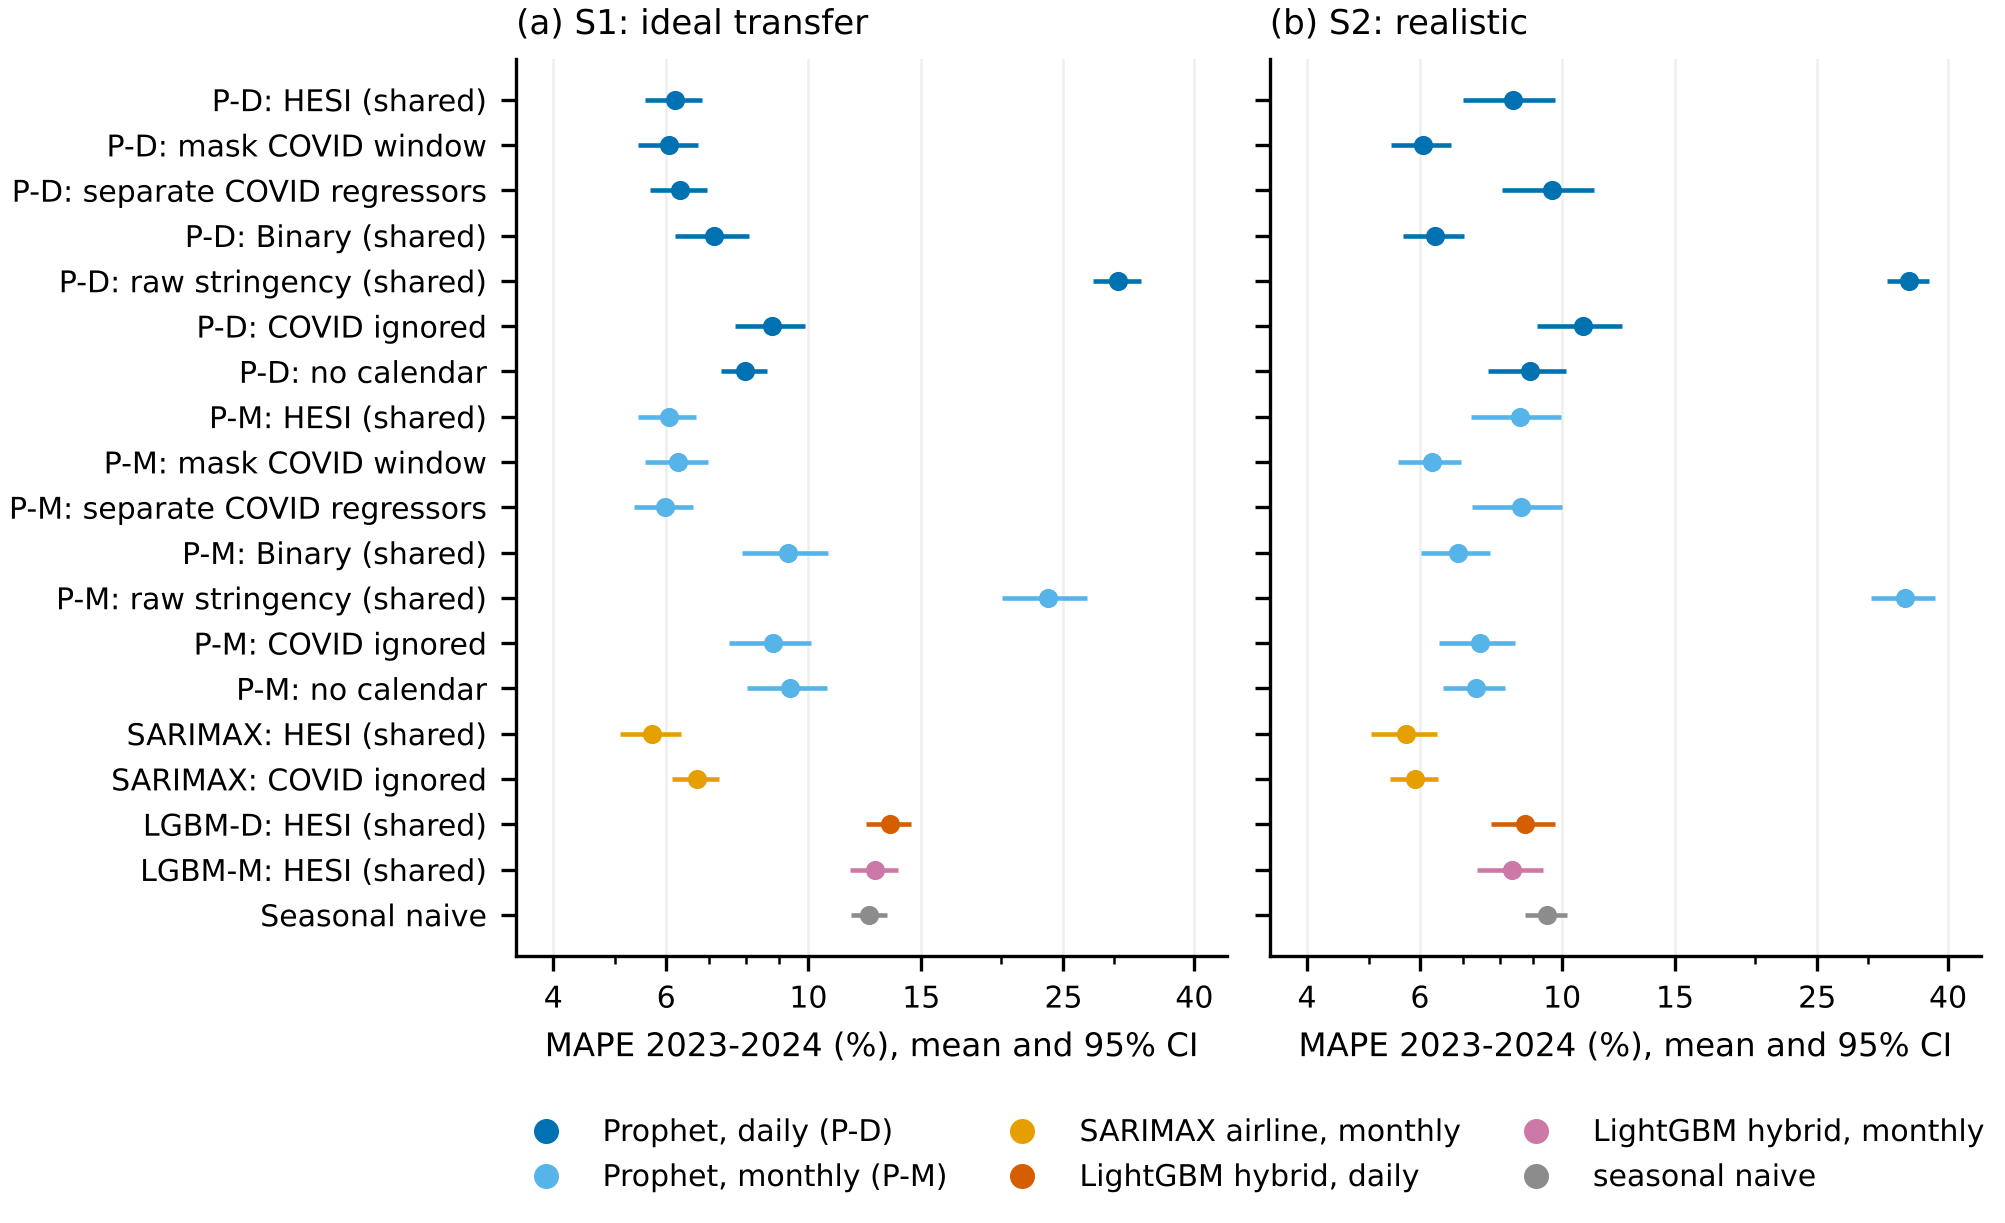
\includegraphics[width=\linewidth]{fig_e2.png}
\caption{Aftermath forecasts (E2): mean MAPE for 2023--2024 with 95\% confidence intervals across replications, logarithmic horizontal axis. Marker colours identify method families: blue for daily Prophet, sky blue for monthly Prophet, orange for SARIMAX, vermilion for daily LightGBM, lilac for monthly LightGBM and grey for the seasonal naive benchmark. Row labels give the treatment of the pandemic in the training sample.}
\label{fig:e2}
\end{figure}

\subsection{Normal times (E0)}
In the absence of a shock (Table~\ref{tab:e0}), daily LightGBM is the most accurate method (<<e0.ld>>\%), followed by monthly LightGBM (<<e0.lm>>\%) and SARIMAX (<<e0.sx>>\%). Daily Prophet with holiday regressors (<<e0.pd>>\%) is close to the seasonal naive benchmark (<<e0.sn>>\%), and the holiday regressors improve it only marginally (from <<e0.pdv>>\%). The value of HES lies in transfer during shocks, not in the general accuracy of Prophet.

\begin{table}[t]
\centering\small
\caption{Normal period (E0, January 2018--December 2019): MAPE (\%) with Monte Carlo standard errors and mean MASE.}
\label{tab:e0}
\begin{tabular}{llcc}
\toprule
Method & Specification & MAPE & MASE \\
\midrule
%%TAB_E0%%
\bottomrule
\end{tabular}
\end{table}

\subsection{Paired inference}
Table~\ref{tab:paired} collects the paired comparisons behind the conclusions above. In S1, the contrasts that establish transfer---HESI against no dose, against the whole-month switch and against raw stringency, and the calibrated dose against no dose---are large relative to their confidence intervals and remain significant after Holm's correction. So do the advantage of daily Prophet over daily LightGBM in both scenarios, the advantage of masking or HESI over ignoring the pandemic in E2, and the advantage of daily LightGBM in normal times. In S2 the evidence for transfer is weaker: HESI and the calibrated dose improve on the no-dose forecast on average, but neither improvement survives Holm's correction (adjusted $p$ = <<ph.c1.s2>> and <<ph.c4.s2>>), whereas calibration significantly improves on the uncalibrated dose (adjusted $p$ = <<ph.c5.s2>>). Several secondary contrasts are not significant after adjustment, including daily Prophet against SARIMAX in S1 (<<ph.c7.s1>>), the aggregation correction in S1 (<<ph.c9.s1>>) and SARIMAX against masking in E2 (<<ph.c12.s1>> and <<ph.c12.s2>>); they should not be over-interpreted.

\begin{table}[!tb]
\centering
\caption{Paired comparisons across <<nseeds>> replications. $\Delta$ is the mean difference in MAPE (method A minus method B, percentage points) with a 95\% $t$-interval; negative values favour A. ``A better'' is the share of replications in which A has the lower MAPE. $p$-values are from the Wilcoxon signed-rank test, unadjusted and Holm-adjusted across all comparisons in the table.}
\label{tab:paired}
\scriptsize
\setlength{\tabcolsep}{3.5pt}
\begin{tabular}{lllcccc}
\toprule
Exp. & Comparison (A vs.\ B) & Scen. & $\Delta$ [95\% CI] & A better & $p$ & Holm $p$ \\
\midrule
%%TAB_PAIRED%%
\bottomrule
\end{tabular}
\end{table}

\section{Discussion}\label{sec:discussion}
\subsection{What transfers, and what does not}
The evidence supports the central hypothesis with qualifications. Elasticities identified on recurring holidays transfer to lockdowns when three conditions hold: the shock is expressed as a dose rather than a switch; the elasticity is estimated at a frequency at which holidays are identified, or the monthly estimate is corrected for aggregation; and the dose scale is either known or calibrated on early data. When these conditions fail, the transfer degrades predictably: an overstated dose produces the right-hand branch of the U-curve, a monthly elasticity produces attenuation, and a tree ensemble produces saturation. The framework is also informative about its own failure: the calibrated dose absorbs coincident demand shocks (Proposition~\ref{prop:transfer}(b)), so a calibrated $\hat\lambda$ far from plausible pass-through values signals that the shock is not primarily a stoppage.

\subsection{A protocol for official Thai export data}\label{sec:protocol}
\begin{enumerate}
\item Use monthly merchandise exports excluding gold as the main series and record the data vintage.
\item Build the observed holiday calendar and the Chinese-New-Year windows.
\item Construct HESI from the Google Community Mobility Reports, with separate references for festivals and ordinary holidays (two-tier specification), and use episode indices or better proxies for China, never raw stringency.
\item With daily or weekly customs data, use daily Prophet with shared regressors; otherwise use monthly Prophet with the aggregation correction alongside SARIMAX.
\item Calibrate the dose on months whose figures have been published, and report the uncertainty of $\hat\lambda$.
\item For the aftermath, compare masking, HESI and SARIMAX by rolling-origin evaluation \citep{tashman2000out}, with Diebold--Mariano tests and the small-sample correction of \citet{harvey1997testing}.
\item Report scenario-conditional forecasts separately from ex-ante forecasts.
\end{enumerate}

\subsection{Threats to validity}
\emph{Internal validity.} In S1 the data-generating process satisfies the assumptions of the framework by construction, which favours HES. Scenario S2, the robustness mechanisms and the dose sweep relax these assumptions in controlled ways, but other departures are possible. \emph{Construct validity.} Workplace mobility measures attendance, not production; the holiday reference is a modelling choice; the Chinese episodes are stylised; and MAPE emphasises relative errors in low-value months. \emph{External validity.} The export series is simulated and its parameters are calibrated rather than estimated; official exports also contain gold, price and exchange-rate movements; and the study covers one economy. \emph{Statistical conclusion validity.} With <<nseeds>> replications, Monte Carlo standard errors are small relative to the main effects but not to all secondary contrasts, which Table~\ref{tab:paired} makes explicit. Prediction intervals were not evaluated.

\subsection{Directions for future research}
The most important next step is the application to official Thai export statistics and, where available, to daily customs records. Further directions include festival-specific dose references; a Bayesian prior on the pass-through $\kappa$ that is updated as data are published; hierarchical models by product and destination; hybrid estimators in which a tree ensemble is trained on the residual after removing the shared stoppage effect, combining the transfer of HES with the accuracy of trees in normal times; and applications to other economies with long festivals, such as the Vietnamese Tet.

\section{Conclusion}\label{sec:conclusion}
Treating lockdowns as partial holidays turns an unforecastable shock into a measurable dose of a familiar event. When the work-stoppage elasticity is identified on recurring holidays through a shared regressor and the pandemic is expressed in holiday units, a forecasting model can anticipate the effect of a lockdown without observing one. The theory developed here explains when this works and how it fails: through the dose scale, through temporal aggregation and through the piecewise-constant structure of tree ensembles. The simulation evidence confirms the theory quantitatively. The approach is not a substitute for adaptive models in normal times or after a shock has passed; it is a structured way to use the knowledge contained in every holiday of the past when the economy stops in an unprecedented way.

\section*{Data and code availability}
The code is distributed with this preprint as ancillary files. The file \texttt{hesi\_forecast.py} reproduces all results with \texttt{python hesi\_forecast.py simulate --reps 30}; \texttt{robust\_en.py} runs the robustness experiments and \texttt{figs\_en.py} the figures, including an automated check that no text in any figure overlaps other text or data areas. The command \texttt{python hesi\_forecast.py real --exports exports.csv} applies the monthly methods to official data (columns \texttt{month,value}), downloading OxCGRT and Google Mobility data automatically. All numbers in the text and tables are generated from the result files.

% NOTE TO AUTHOR: the bibliographic entries below were compiled without database access.
% Verify every entry (authors, year, title, venue, volume, pages, DOI) before submission.
\begin{thebibliography}{99}
\setlength{\itemsep}{1pt}\small
\bibitem[Bai and Perron(1998)]{bai1998multiple} Bai, J., \& Perron, P. (1998). Estimating and testing linear models with multiple structural changes. \emph{Econometrica}, 66(1), 47--78.
\bibitem[Baldwin and Tomiura(2020)]{baldwin2020trade} Baldwin, R., \& Tomiura, E. (2020). Thinking ahead about the trade impact of COVID-19. In R. Baldwin \& B. Weder di Mauro (Eds.), \emph{Economics in the Time of COVID-19} (pp.\ 59--71). CEPR Press.
\bibitem[Bell and Hillmer(1983)]{bell1983calendar} Bell, W. R., \& Hillmer, S. C. (1983). Modeling time series with calendar variation. \emph{Journal of the American Statistical Association}, 78(383), 526--534.
\bibitem[Box and Tiao(1975)]{box1975intervention} Box, G. E. P., \& Tiao, G. C. (1975). Intervention analysis with applications to economic and environmental problems. \emph{Journal of the American Statistical Association}, 70(349), 70--79.
\bibitem[Box et~al.(2015)]{box2015time} Box, G. E. P., Jenkins, G. M., Reinsel, G. C., \& Ljung, G. M. (2015). \emph{Time Series Analysis: Forecasting and Control} (5th ed.). Wiley.
\bibitem[Breiman et~al.(1984)]{breiman1984cart} Breiman, L., Friedman, J. H., Olshen, R. A., \& Stone, C. J. (1984). \emph{Classification and Regression Trees}. Wadsworth.
\bibitem[Chen and Liu(1993)]{chen1993joint} Chen, C., \& Liu, L.-M. (1993). Joint estimation of model parameters and outlier effects in time series. \emph{Journal of the American Statistical Association}, 88(421), 284--297.
\bibitem[Chow and Lin(1971)]{chow1971interpolation} Chow, G. C., \& Lin, A. (1971). Best linear unbiased interpolation, distribution, and extrapolation of time series by related series. \emph{Review of Economics and Statistics}, 53(4), 372--375.
\bibitem[Clements and Hendry(1998)]{clements1998forecasting} Clements, M. P., \& Hendry, D. F. (1998). \emph{Forecasting Economic Time Series}. Cambridge University Press.
\bibitem[Cleveland and Devlin(1982)]{cleveland1982calendar} Cleveland, W. P., \& Devlin, S. J. (1982). Calendar effects in monthly time series: Modeling and adjustment. \emph{Journal of the American Statistical Association}, 77(379), 520--528.
\bibitem[Denton(1971)]{denton1971adjustment} Denton, F. T. (1971). Adjustment of monthly or quarterly series to annual totals: An approach based on quadratic minimization. \emph{Journal of the American Statistical Association}, 66(333), 99--102.
\bibitem[Diebold and Mariano(1995)]{diebold1995comparing} Diebold, F. X., \& Mariano, R. S. (1995). Comparing predictive accuracy. \emph{Journal of Business \& Economic Statistics}, 13(3), 253--263.
\bibitem[Duan(1983)]{duan1983smearing} Duan, N. (1983). Smearing estimate: A nonparametric retransformation method. \emph{Journal of the American Statistical Association}, 78(383), 605--610.
\bibitem[Findley et~al.(1998)]{findley1998x12} Findley, D. F., Monsell, B. C., Bell, W. R., Otto, M. C., \& Chen, B.-C. (1998). New capabilities and methods of the X-12-ARIMA seasonal-adjustment program. \emph{Journal of Business \& Economic Statistics}, 16(2), 127--152.
\bibitem[Foroni et~al.(2022)]{foroni2022covid} Foroni, C., Marcellino, M., \& Stevanovic, D. (2022). Forecasting the Covid-19 recession and recovery: Lessons from the financial crisis. \emph{International Journal of Forecasting}, 38(2), 596--612.
\bibitem[Friedman(2001)]{friedman2001greedy} Friedman, J. H. (2001). Greedy function approximation: A gradient boosting machine. \emph{Annals of Statistics}, 29(5), 1189--1232.
\bibitem[Ghysels et~al.(2007)]{ghysels2007midas} Ghysels, E., Sinko, A., \& Valkanov, R. (2007). MIDAS regressions: Further results and new directions. \emph{Econometric Reviews}, 26(1), 53--90.
\bibitem[Google LLC(2022)]{google2022mobility} Google LLC. (2022). \emph{Google COVID-19 Community Mobility Reports}. \url{https://www.google.com/covid19/mobility/}
\bibitem[Grinsztajn et~al.(2022)]{grinsztajn2022tree} Grinsztajn, L., Oyallon, E., \& Varoquaux, G. (2022). Why do tree-based models still outperform deep learning on typical tabular data? In \emph{Advances in Neural Information Processing Systems 35, Datasets and Benchmarks Track}.
\bibitem[Hale et~al.(2021)]{hale2021oxcgrt} Hale, T., Angrist, N., Goldszmidt, R., et~al. (2021). A global panel database of pandemic policies (Oxford COVID-19 Government Response Tracker). \emph{Nature Human Behaviour}, 5, 529--538.
\bibitem[Harvey et~al.(1997)]{harvey1997testing} Harvey, D., Leybourne, S., \& Newbold, P. (1997). Testing the equality of prediction mean squared errors. \emph{International Journal of Forecasting}, 13(2), 281--291.
\bibitem[Hastie et~al.(2009)]{hastie2009elements} Hastie, T., Tibshirani, R., \& Friedman, J. (2009). \emph{The Elements of Statistical Learning} (2nd ed.). Springer.
\bibitem[Hyndman and Athanasopoulos(2021)]{hyndman2021fpp} Hyndman, R. J., \& Athanasopoulos, G. (2021). \emph{Forecasting: Principles and Practice} (3rd ed.). OTexts.
\bibitem[Hyndman and Koehler(2006)]{hyndman2006another} Hyndman, R. J., \& Koehler, A. B. (2006). Another look at measures of forecast accuracy. \emph{International Journal of Forecasting}, 22(4), 679--688.
\bibitem[Januschowski et~al.(2022)]{januschowski2022trees} Januschowski, T., Wang, Y., Torkkola, K., Erkkilä, T., Hasson, H., \& Gasthaus, J. (2022). Forecasting with trees. \emph{International Journal of Forecasting}, 38(4), 1473--1481.
\bibitem[Ke et~al.(2017)]{ke2017lightgbm} Ke, G., Meng, Q., Finley, T., Wang, T., Chen, W., Ma, W., Ye, Q., \& Liu, T.-Y. (2017). LightGBM: A highly efficient gradient boosting decision tree. In \emph{Advances in Neural Information Processing Systems 30}.
\bibitem[Lenza and Primiceri(2022)]{lenza2022var} Lenza, M., \& Primiceri, G. E. (2022). How to estimate a vector autoregression after March 2020. \emph{Journal of Applied Econometrics}, 37(4), 688--699.
\bibitem[Lin and Liu(2003)]{lin2003lunar} Lin, J.-L., \& Liu, T.-S. (2003). Modeling lunar calendar holiday effects in Taiwan. \emph{Taiwan Economic Forecast and Policy}, 33(2), 1--37.
\bibitem[Makridakis et~al.(2022)]{makridakis2022m5} Makridakis, S., Spiliotis, E., \& Assimakopoulos, V. (2022). M5 accuracy competition: Results, findings, and conclusions. \emph{International Journal of Forecasting}, 38(4), 1346--1364.
\bibitem[Meta(n.d.)]{prophetshocks} Meta Open Source. (n.d.). Handling shocks. \emph{Prophet documentation}. \url{https://facebook.github.io/prophet/docs/handling_shocks.html}
\bibitem[Morris et~al.(2019)]{morris2019simulation} Morris, T. P., White, I. R., \& Crowther, M. J. (2019). Using simulation studies to evaluate statistical methods. \emph{Statistics in Medicine}, 38(11), 2074--2102.
\bibitem[Perron(1989)]{perron1989crash} Perron, P. (1989). The great crash, the oil price shock, and the unit root hypothesis. \emph{Econometrica}, 57(6), 1361--1401.
\bibitem[Pesaran and Timmermann(2007)]{pesaran2007window} Pesaran, M. H., \& Timmermann, A. (2007). Selection of estimation window in the presence of breaks. \emph{Journal of Econometrics}, 137(1), 134--161.
\bibitem[python-holidays contributors(2025)]{pyholidays} python-holidays contributors. (2025). \emph{holidays: Open World Holidays Framework} [Software]. \url{https://github.com/vacanza/holidays}
\bibitem[Rossi(2013)]{rossi2013instability} Rossi, B. (2013). Advances in forecasting under instability. In G. Elliott \& A. Timmermann (Eds.), \emph{Handbook of Economic Forecasting} (Vol.\ 2B, pp.\ 1203--1324). Elsevier.
\bibitem[Sampi and Jooste(2020)]{sampi2020nowcasting} Sampi, J., \& Jooste, C. (2020). Nowcasting economic activity in times of COVID-19: An approximation from the Google Community Mobility Report. \emph{World Bank Policy Research Working Paper}, 9247.
\bibitem[Silvestrini and Veredas(2008)]{silvestrini2008aggregation} Silvestrini, A., \& Veredas, D. (2008). Temporal aggregation of univariate and multivariate time series models: A survey. \emph{Journal of Economic Surveys}, 22(3), 458--497.
\bibitem[Stock and Watson(1996)]{stock1996instability} Stock, J. H., \& Watson, M. W. (1996). Evidence on structural instability in macroeconomic time series relations. \emph{Journal of Business \& Economic Statistics}, 14(1), 11--30.
\bibitem[Tashman(2000)]{tashman2000out} Tashman, L. J. (2000). Out-of-sample tests of forecasting accuracy: An analysis and review. \emph{International Journal of Forecasting}, 16(4), 437--450.
\bibitem[Taylor and Letham(2018)]{taylor2018forecasting} Taylor, S. J., \& Letham, B. (2018). Forecasting at scale. \emph{The American Statistician}, 72(1), 37--45.
\bibitem[Wilcoxon(1945)]{wilcoxon1945individual} Wilcoxon, F. (1945). Individual comparisons by ranking methods. \emph{Biometrics Bulletin}, 1(6), 80--83.
\end{thebibliography}

\appendix
\section{Proofs}\label{app:proofs}
\paragraph{Remark~\ref{rem:oneoff}.} Prophet represents holiday effects as $Z(t)\bm{\kappa}$ with $\kappa_j\sim N(0,\sigma_h^2)$. For a holiday that does not occur in the estimation window, column $j$ of $Z$ is zero for all estimation dates, so the log posterior equals $-\kappa_j^2/(2\sigma_h^2)$ plus terms that do not involve $\kappa_j$. It is maximised at $\kappa_j=0$, and the forecast contribution $Z_j(t)\kappa_j$ is zero for every future date. \qed

\paragraph{Proposition~\ref{prop:transfer}.} On a non-holiday day with $\lambda h_d\le1$ and $z_d\le1$, equation~\eqref{eq:model} gives $\log y_d=m_d+\beta_D\kappa h_d(1+\nu_d)+\beta_P x^P_d+D_d+u_d$ with $m_d=g+s+w$, and the forecast is $\log\hat y_d=\hat m_d+\hat\beta_D\lambda h_d+\hat\beta_P\hat x^P_d$. Subtracting and adding $\beta_D\lambda h_d$ yields~\eqref{eq:error} with $r_d=(m_d-\hat m_d)+(\beta_P x^P_d-\hat\beta_P\hat x^P_d)+D_d+u_d$. Part (a) follows by taking expectations with $\E[\nu_d\mid h_d]=0$. For part (b), with $\hat\beta_D=\beta_D$ and $\nu_d$ independent of $r_d$, $\sum_d\E[e_d^2]=\sum_d\E[\{\beta_D h_d(\kappa-\lambda)+r_d\}^2]+\text{const}$. Setting the derivative with respect to $\lambda$ to zero gives $\beta_D^2(\kappa-\lambda)\sum_d h_d^2+\beta_D\sum_d h_d\E[r_d]=0$, which is~\eqref{eq:lamstar}; the objective is convex in $\lambda$. Part (c) substitutes $\lambda h_d\equiv1$ in the selected months and $\lambda=0$ elsewhere. \qed

\paragraph{Proposition~\ref{prop:jensen}.} Let $X$ be a day drawn from month $m$ with probabilities $w_d$. Then $E_m(\beta)=K(\beta)$, the cumulant generating function of $X$. (a) $K$ is convex with $K(0)=0$ and $K'(0)=\E_w X=\bar x_m$, so $K(\beta)\ge\beta\bar x_m$ (equivalently, Jensen's inequality applied to $e^{\beta X}$), with equality if and only if $X$ is degenerate. (b) is the cumulant expansion $K(\beta)=\beta\kappa_1+\beta^2\kappa_2/2+O(\beta^3)$ with $\kappa_1=\bar x_m$ and $\kappa_2=\operatorname{Var}_w(X)$. (c) If $X\in\{0,1\}$ with $\Pr(X=1)=q$, then $K(\beta)=\log(1-q+qe^{\beta})$. Since $\log(1+u)=u+O(u^2)$, $K(\beta)=q(e^{\beta}-1)+O(q^2)$, and the least-squares slope through the origin, $\sum qK/\sum q^2$, equals $e^{\beta}-1+O(\max q)$. Because $e^{\beta}>1+\beta$ for $\beta\ne0$, $e^{\beta}-1>\beta$, so $|\beta_M|<|\beta|$ when $\beta<0$. (d) A constant dose gives $K(\beta)=\beta c$, and the error of the monthly forecast is $(e^{\beta}-1)c-\beta c=(e^{\beta}-1-\beta)c\ge0$, i.e.\ the forecast effect is smaller in magnitude by $(1+\beta-e^{\beta})|c|$ for $c\ge0$, since $\beta c\le0$. \qed

\paragraph{Corollary~\ref{cor:ac}.} The map $\beta\mapsto e^{\beta}-1$ is strictly increasing with inverse $b\mapsto\log(1+b)$ on $b>-1$. The delta method gives $\operatorname{Var}\{\log(1+\hat\beta_M)\}\approx\operatorname{Var}(\hat\beta_M)/(1+\beta_M)^2$. The minimum-distance version replaces the approximation $q(e^{b}-1)$ by the exact $E_m(b)$ for each month. \qed

\paragraph{Proposition~\ref{prop:ident}.} The Frisch--Waugh--Lovell theorem expresses $\hat\beta_M$ as the slope of the regression of residualised $\log(Y_m/D_m)$ on residualised $\bar x^D_m$; under homoskedastic, uncorrelated errors its variance is $\sigma_m^2/\sum_m\tilde x_m^2$. Holidays with fixed dates contribute the same amount to $\bar x^D_m$ in every year apart from in-lieu adjustments, so their contribution is absorbed by the calendar-month effects and does not enter $\tilde x_m$. In daily data the residual of a holiday indicator after projection on smooth seasonal and day-of-week terms is close to the indicator itself, because a single day has negligible projection on smooth functions of the date. \qed

\paragraph{Proposition~\ref{prop:tree}.} A regression tree splits a feature at thresholds between distinct observed values. With observed values $\{0,1\}$, every threshold lies in $(0,1)$; with histogram binning there is a single bin boundary and hence a single threshold $c$ for all trees. Holding the other features fixed, every tree maps $x\le c$ and $x>c$ to two constants, and so does their sum. For a continuous feature with maximal observed value $a$, no threshold exceeds $a$, so all $x>a$ fall in the same leaves as $x=a$. \qed

\section{Additional results}\label{app:extra}
\begin{table}[h]
\centering
\caption{Shock period (E1): mean MASE over <<nseeds>> replications with Monte Carlo standard errors.}
\label{tab:e1mase}
\scriptsize
\setlength{\tabcolsep}{4pt}
\begin{tabular}{llcccc}
\toprule
 & & \multicolumn{2}{c}{S1: ideal transfer} & \multicolumn{2}{c}{S2: realistic} \\
\cmidrule(lr){3-4}\cmidrule(lr){5-6}
Method & Dose variant & Jan--Dec & May--Dec & Jan--Dec & May--Dec \\
\midrule
%%TAB_E1MASE%%
\bottomrule
\end{tabular}
\end{table}

\section{Implementation details}\label{app:impl}
All computations used Python 3.12 with prophet 1.5.0, lightgbm 4.7.0, statsmodels 0.15.0 \citep{box2015time} and holidays 0.108. Prophet was estimated by maximum a posteriori with default trend priors, regressor prior scale 10 and \texttt{uncertainty\_samples=0}. LightGBM used 400 trees, learning rate 0.05, 31 leaves and 20 observations per leaf for daily data, and 300 trees, learning rate 0.05, 7 leaves and 5 observations per leaf for monthly data. SARIMAX was estimated by maximum likelihood with up to 300 iterations. One replication of all experiments takes about 25--30 seconds on one CPU core; the robustness experiments take about 2--3 seconds per replication.

\section{Code excerpt}\label{app:code}
\begin{lstlisting}
def mobility_hesi(mob, hol, window=7):
    """HESI_d = workplace-mobility drop on day d / median drop on weekday public holidays."""
    drop = (-mob / 100.0).clip(lower=0)
    is_hol = drop.index.isin(hol)
    ref = float(drop[is_hol & (drop.index.dayofweek < 5)].median())
    smooth = drop.where(~is_hol).rolling(window, center=True, min_periods=3).mean()
    return (smooth / ref).clip(0, 1).fillna(0.0), ref

def stoppage_X(cal, drv, variant, lam=1.0):
    """Shared regressors: xD = H + (1-H)*min(1, lam*HESI);  xP = C + (1-C)*episode."""
    H, C = cal.H.values, cal.C.values
    zD, zP = np.zeros(len(cal)), np.zeros(len(cal))
    if variant == "binary":       zD, zP = drv.bin_th.values, drv.bin_cn.values
    elif variant == "stringency": zD, zP = drv.s_th.values, drv.s_cn.values
    elif variant == "hesi":       zD, zP = lam * drv.hesi_th.values, drv.e_cn.values
    zD, zP = np.clip(zD, 0, 1), np.clip(zP, 0, 1)
    return pd.DataFrame({"xD": H + (1 - H) * zD, "xP": C + (1 - C) * zP}, index=cal.index)

def deaggregate_beta(beta_m, x_train, grid=np.linspace(-3.0, 0.0, 601)):
    """Aggregation correction: daily beta whose monthly log-mean-exp matches beta_m * mean(x)."""
    Mx = month_matrix(x_train)                       # months x days (NaN padded)
    target = beta_m * np.nanmean(Mx, axis=1)
    E = np.log(np.nanmean(np.exp(grid[:, None, None] * Mx[None]), axis=2))
    return float(grid[np.argmin(((E - target[None]) ** 2).sum(axis=1))])
\end{lstlisting}
\end{document}
